\chapter{Elements of Audio Signal Processing}\label{ch:processing}
\openepigraph{Signal, a function that conveys information about a phenomenon.
$[\dots]$ Consider an acoustic wave, which can convey acoustic or music information.}{R. Priemer, \textit{Introductory Signal Processing}}
\vspace{-2.5em}
\newthought{Synopsis}\synopsisChProcessing
\\Unless specified, the notation and definitions presented in this chapter for the audio signal model are excerpted from~\citeauthor{vincent2018audio}'s book \textit{Audio source separation and speech enhancement}.
The material used for illustrating concepts of digital signal processing are taken from standard book on the topics.

\section{Signal model in the time domain}\label{sec:processing:model}
In the previous chapter we formalized the physics that rule the sound propagation from the source to the microphone.
A raw \textit{audio signal} encodes the variation of pressure over time on the microphone membrane.
Mathematically it is denoted as the function
\begin{equation}
    \begin{aligned}
        \tildex : \bbR &\kto \bbR\\
                     t &\kmapsto \tilde{x}(t),
    \end{aligned}
\end{equation}
continuous both in time $t \in \R$ and amplitudes.
\marginpar{
    \centering
    \footnotesize
    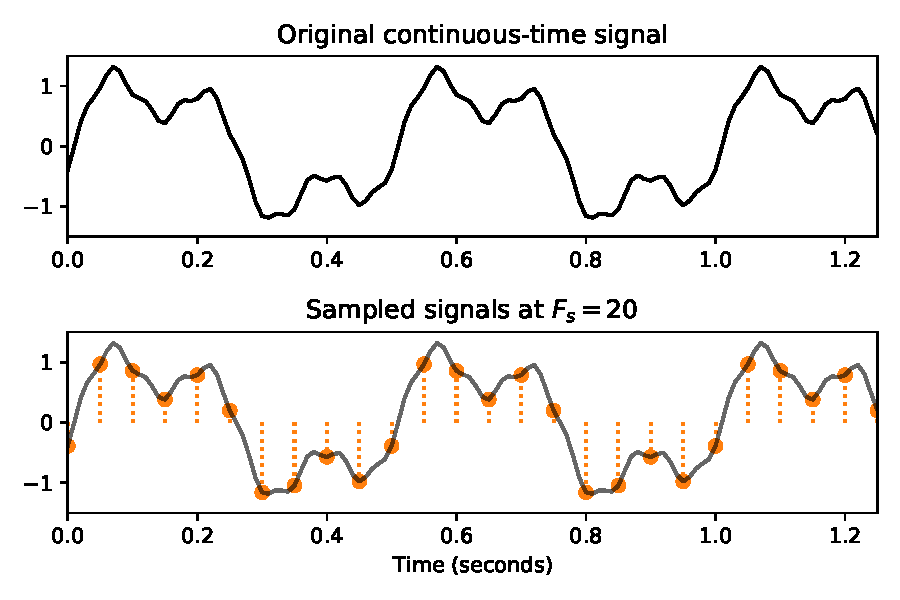
\includegraphics[width=\linewidth]{processing/py_processing.pdf}
    \captionof{figure}{Continuous-time signal and its sampled version.}
    \label{fig:processing:sampling}
}

\mynewline
Today signals are typically processed, stored and analyzed by computers as \textit{digital audio signal}.
This corresponds to finite and discrete-time signal $x_\idxSample$ obtained by periodically sampling the continuous-time signal $\tilde{x}$ at rate $\Fs\;[\si{\Hz}]$, truncate it to $\idxSample$ samples.
\marginpar{
    \footnotesize
    Strickly speaking, the digital representation of a continuos signal involves sampling and quantization.
    In this thesis we assume the sampled signals are real-valued, ignoring the \textit{quantization} process.}
As common to most measurement models, we assume that the sampling process involves two steps:
first, the impinging signal undergoes an ideal low-pass filter $\lowpassfilter$ with frequency support in $\kintervoc{\sfrac{-\Fs}{2}}{\sfrac{\Fs}{2}}$\sidenote{
    The ideal low-pass filter is\\$\lowpassfilter(t) = \sinc(t) = \sin(\pi \Fs t) / (\pi \Fs t)$.
    \\The term sinc stands for \textit{sinus cardinal} and was introduced by Philip M. Woodward in 1952 in~\citeonly{woodward1952information},
    in which he said that the function "\textit{occurs so often in Fourier analysis and its applications that it does seem to merit some notation of its own}"
}; then it time-support is regularly discretized, $t = n/\Fs$ for $n \in \Z$.
This is expressed by
\begin{equation}
    \discTime[\idxSample]{\mic} = \kparen{\lowpassfilter \convCont \tilde{x}}\kparen{\frac{n}{\Fs}} \in \R
    ,
\end{equation}
where $\convCont$ is the continuous-time convolution operator.
This will restrict the frequency support of signal to satisfy the \textit{Nyquist–Shannon sampling theorem} and avoid aliasing effect.

\mynewline
Finally, at the end of the discretisation process, the $\tilde{x}(t)$ is represented as the finite time series or a vector,
\begin{equation}
    \hat{\mic}_{\numSample} \in \R^{\numSample}
    ,
\end{equation}
with entries $\hat{\mic}_{\numSample}[\idxSample]$ for $n = 0, \ldots, \numSample-1$.

\mynewline
The choice of $\Fs$ depends on the application since it is a trade-off between computational power, processing and rendering quality.
Historically the two iconic values are $\SI{44.1}{\kHz}$ for music distribution on CDs and $\SI{8}{\kHz}$ for first-generation speech communication.
Now multiples of $\SI{8}{\kHz}$ are typically used in audio processing: ($16, 48, 96, \SI{128}{\kHz}$).

\mynewline
Audio signals are emitted by sources and are observed, received or recorded by microphones.
A set of microphones is called a microphone \textit{array}, whose signals are sometime referred to as \textit{channels}.
In this thesis, these objects are assumed to have been deployed in a indoor environment, called generically \textit{room}.
Let us provide some taxonomy, through some dichotomies, useful for describe the mixing process later:

\dichotomy{Sources \vs/ Mixtures:}
Sound sources emits sounds.
When multiple sources are active at the same time, the sounds that reach our ears or are recorded by microphones are superimposed or \textit{mixed} into a single sound.
This resulting signal is denoted as \textit{mixture}.

\dichotomy{Single-Channel \vs/ Multichannel:}
The term \textit{channel}
% \sidenote{%
%     Please note, the term \textit{channel} has also different meaning:
%     it indicates the medium in communication (\eg/ Channel Estimation)
%     and sometimes one of the dimension of the input in machine learning (\eg/ image's channel).
% }
is used here to indicate the output of one microphones or one source.
A \textit{single-channel} signal ($\numMics = 1$) is represented by the scalar $\tilde{\mic}(t) \in \R$,
while a \textit{multichannel} ($\numMics >   1$) is represented by the vector $\tilde{\mics}(t) = \ktranspose{\klist{\tilde{\mic}_1, \dots, \tilde{\mic}_{\numMics}}} \in \R^{\numMics}$.

\dichotomy{Point \vs/ Diffuse Sources:}
\textit{Point sources} are single and well-defined points in the space emitting single-channel signal.
In certain application, human speakers or the sound emitted by a loudspeaker can be reasonably modeled as in this way.
\\\textit{Diffuse sources} refers for instance to wind, traffic noise, or large musical instruments, which emit sound in a large region of space.
Their sound cannot be associate to a punctual source, but rather a distributed collection of them.

\dichotomy{Directional \vs/ Onmidirectional:}
An \textit{omnidirectional} source (\resp/ receiver) will in principle emit (\resp/ record) sound equally from all directions,
both in time and in frequency.
Although this greatly simplifies processing models and frameworks, this is not true in real scenario.
The physical properties of real sources (\resp/ receivers) leads to \textit{directivity patterns}, \aka/ \textit{polarity}, which may
be different at different frequencies.
In this thesis we will assume omnidirectional sources and receivers.

\subsection{The mixing process}\label{subsec:processing:mixing}
Let us assume the observed signal has $\numMics$ \textit{channels} indexed by $\idxMic \in \kbrace{1,\dots,\numMics}$.
Let us assume that there are $\numSrcs$ sources indexed by $\idxSrc \in \kbrace{1,\dots,\numSrcs}$.
Each microphone $\idxMic$ and each source $\idxSrc$ have a well defined position in the space, $\positionMicrophone_\idxMic$, $\positionSource_\idxSrc$, respectively.

The mixing process describes then the nature of the mixtures.
In order to better formalized it, the authors of \citeonly{sturmel2012linear} introduced the intermediate representation called \emph{source spatial images}:
$\tilde{\img}_{\idxMic\idxSrc}(t)$ describes the contribution of the source $\idxSrc$ to the microphone $\idxMic$.
Consequently, the \textit{mixture} $\tilde{\mic}_{\idxSrc}$ is the combination of images associated to the source $j$.
Depending on the ``contribution'' the image describes, the following type of mixture can be defined:

\dichotomy{Natural \vs/ Artificial Mixtures:}
The former refers to microphone mixtures recorded simultaneously the same auditory scene, \eg/ teleconferencing systems or hands-free devices.
By contrast, the latters are created by mixing together different individual, possibly processed, recordings.
This are the typical mixtures used professional music production where the usage of long-chain of audio effects typically ``hide'', willingly or not, the recording environment of the sound sources.

\dichotomy{Instantaneous \vs/ Convolutive Mixtures:}
In the first case, the mixing process boils down to a simple linear combination of the source signals, namely
the mixing filters are just scalar factors.
This is the typical scenario when sources are mixed using a mixing console.
\marginpar{%
    \footnotesize
    \centering
    \begin{tabular}{p{0.33\linewidth}|p{0.66\linewidth}}
    \toprule
    instantaneous   & $\tilde{\img}_ij =a_{ij} \tilde{\src}(t) $ \\
    anechoic        & $\tilde{\img}_ij =a_{ij} \tilde{\src}_j (t - \tau_{ij})$ \\
    convolutive     & $\tilde{\img}_ij =(\tilde{g}_{ij} \convCont \tilde{\src}_j) (t)$ \\
    \bottomrule
    \end{tabular}
    \captionof{table}{Taxonomy of linear mixing models for a mixture channel $x_i$,
    sources $\src_j$, impulse response $\tilde{g}_{ij}$, scaling factor $a_{ij}$ and delay $\tau_{ij}$.}
}
Convolutive mixtures, instead, denote the more general case where the each mixture is the sum of filtered signals.
In between are the \textit{anechoic} mixtures involving the sum of scaled and delayed source signals.
Natural mixtures are convolutive by nature and ideal free-far-field natural recording are well approximated by anechoic mixtures.

\begin{figure}[t]
    \begin{fullwidth}
        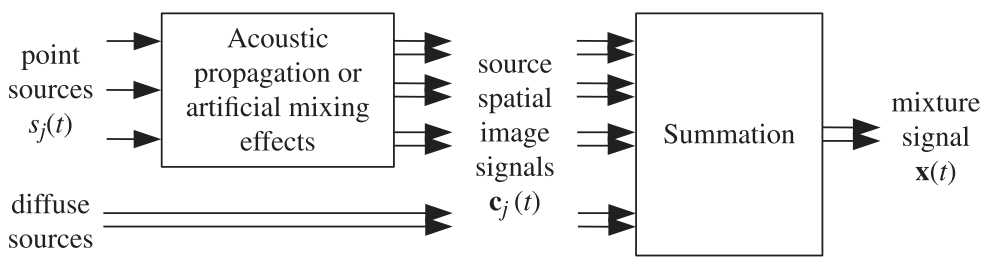
\includegraphics[width=\linewidth+\marginparsep]{processing/mixing_process.png}

        \caption{General mixing process, illustrated in the case of $\numSrcs = 3$ sources,
        including three point sources and one diffuse source, and $\numMics = 2$ channels.}

        \label{fig:processing:mixing}
    \end{fullwidth}
\end{figure}

\newthought{In this thesis}, we will particularly focus on natural mixture:
the microphone mixture listens to the propagation of sound in the room and this process is linear (\cfr{\cref{ch:acoustics:sec:wave}}) and time invariant provided a static scenario.
% In this case, the spatialization operation $\spat_\idxSrc(\cdot)$ is expressed by
% collection of convolution with \RIR/ $h_{\idxMic\idxSrc}$
% from source $\idxSrc$ to microphone $\idxMic$ and the post-mixing operation $\master(\cdot)$ reduces to the identity:
Therefore, the resulting mixture is the simple summation of the sound images,
which are the collections of convolution between the \RIRs/ and source signal:
\marginpar{
    \centering
        \tikzset{every picture/.style={line width=0.75pt}} %set default line width to 0.75pt
        \resizebox{\linewidth}{!}{
            \begin{tikzpicture}[x=0.75pt,y=0.75pt,yscale=-1,xscale=1]

    % Picture Node
    \draw (333,148.65) node  {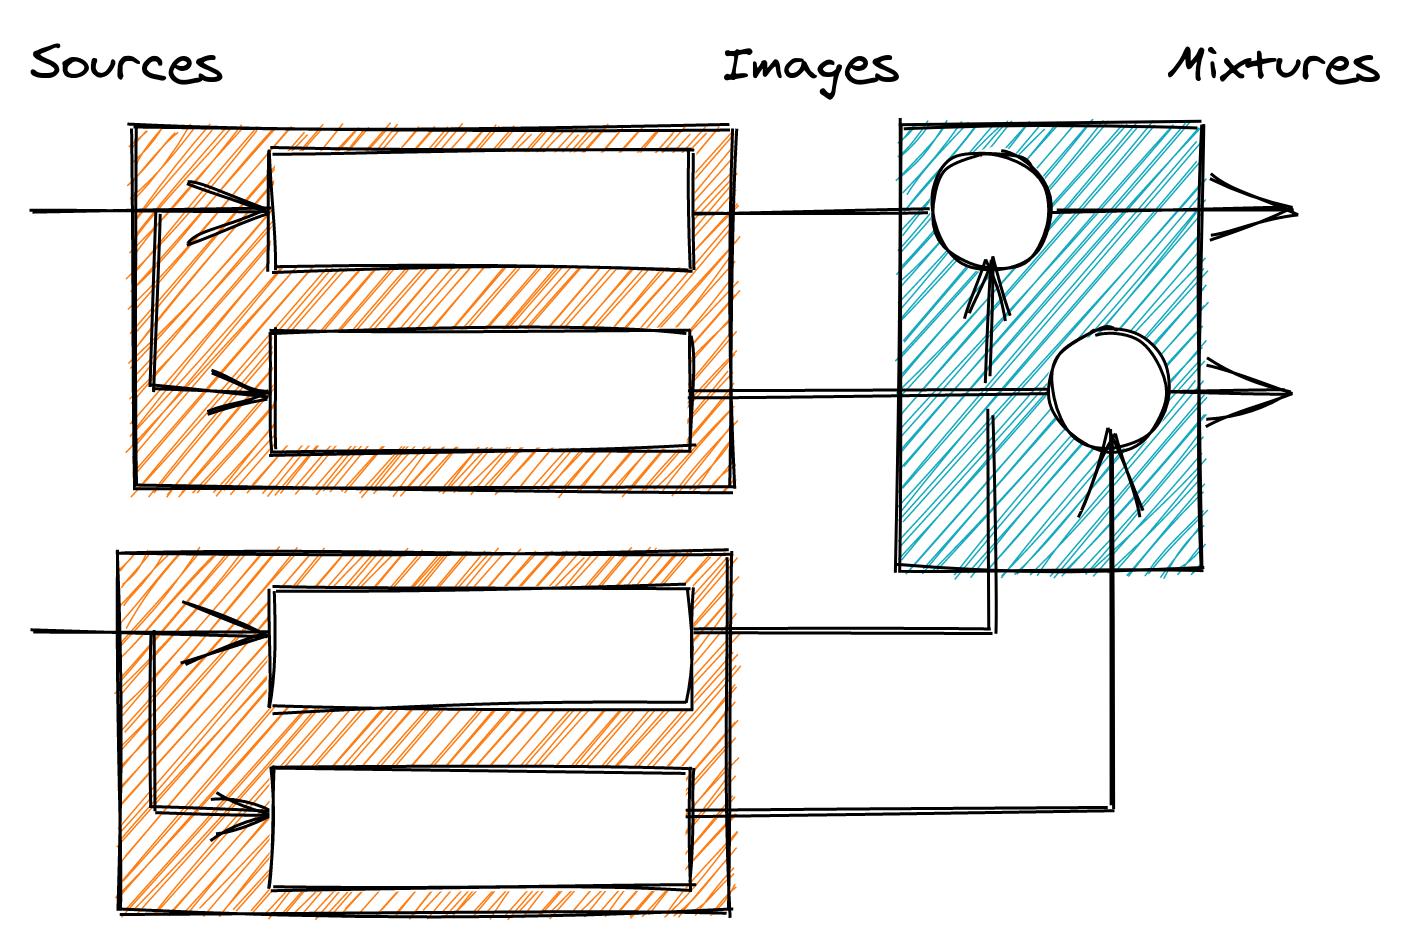
\includegraphics[width=333.75pt,height=222.97pt]{processing/mixing_blocks.png}};

    % Text Node
    \draw (126,53) node [font=\huge]   {$s_{1}$};
    % Text Node
    \draw (126,183) node  [font=\huge]  {$s_{2}$};
    % Text Node
    \draw (262,63) node  [font=\huge]  {$h_{11} \ast s_{1}$};
    % Text Node
    \draw (262,120) node  [font=\huge]  {$h_{21} \ast s_{1}$};
    % Text Node
    \draw (370,53) node  [font=\huge]  {$c_{11}$};
    % Text Node
    \draw (370,110) node [font=\huge]   {$c_{21}$};
    % Text Node
    \draw (530,53) node   [font=\huge] {$x_{1}$};
    % Text Node
    \draw (530,110) node  [font=\huge]  {$x_{2}$};
    % Text Node
    \draw (262,199) node  [font=\huge]  {$h_{12} \ast s_{2}$};
    % Text Node
    \draw (262,256) node  [font=\huge]  {$h_{22} \ast s_{2}$};
    % Text Node
    \draw (370,183) node  [font=\huge]  {$c_{12}$};
    % Text Node
    \draw (370,240) node   [font=\huge] {$c_{22}$};
    % Text Node
    \draw (412,53) node [anchor=north west][inner sep=0.75pt]  [font=\huge]  {$\sum $};
    % Text Node
    \draw (448,109) node [anchor=north west][inner sep=0.75pt]  [font=\huge]  {$\sum $};

\end{tikzpicture}
        }
        \captionof{figure}{Graphical representation of the mixing model~\ref{eq:processing:mixing:mix} for 2 sources and 2 microphones.}\label{fig:processing:mixing}
}
\begin{align}
    \tilde{\img}_{\idxMic\idxSrc}(t) &= \kparen{\tilde{\rir}_{\idxMic\idxSrc} \convCont \tilde{\src}_\idxSrc} (t)     \label{eq:processing:mixing:img} \\
    \tilde{\imgs}_\idxSrc(t)         &= \ktranspose{\klist{\tilde{\img}_{1\idxSrc}(t), \dots, \tilde{\img}_{\numMics\idxSrc}(t)}} \nonumber\\
    \tilde{\mics}(t)                 &= \sum_{\idxSrc=1}^{\numSrcs} \tilde{\imgs}_\idxSrc(t)                    \label{eq:processing:mixing:mix}
    .
\end{align}%
Considering the time domain description of the \RIR/ derived (and approximated) in the previous chapter,
the time-domain \emph{mixing filters} $\tilde{h}_{ij}( t)$ will be modeled as follows:
\begin{equation}\label{eq:processing:mixing_filter}
    \tilde{h}_{ij}( t) = \sum_{\idxEch=0}^{\numEchs} \frac{\absCoeff_{ij}^r}{4 \pi \speedOfSound \tau_{ij}^r}
                          \diracOf{t - \tau_{ij}^r} + \varepsilon_{ij}(t)
\end{equation}
where $\absCoeff_{ij}^r \in \R$ and $\tau_{ij}^r \in \R$ are the attenuation coefficient and the time delay of the reflection $\idxEch$.
The noise term $\tilde{\varepsilon}_{ij}( t)$ collects later echoes ($\idxEch > \numEchs$) and the tail of the reverberation.
We do not assume $\tilde{\varepsilon}_{ij}( t)$ to be known.

\subsection{Noise, interferer and errors}
% \openepigraph{%
%     \emph{Noise} is a general term for unwanted (and, in general, unknown) modifications that a signal may suffer during capture, storage, transmission, processing, or conversion
% }{V. Tuzlukov, \textit{Signal processing noise}}
In~\cref{eq:processing:mixing:mix} no noise is included:
all the sources are threated in the same way, including \textit{target}, \textit{interfering} and \textit{noise} sources.
While the definition of target sound source is quite self-explanatory and it will denoted by default as the first source, that is $j = 1$,
the term interfer and noise depends on the specific use case, problem, application, and research field.
Notice that in~\cref{eq:processing:mixing_filter} a noise term is added to gather unknown quantities.
\begin{quote}
    \textit{Noise is a general term for unwanted (and, in general, unknown) modifications that a signal may suffer during capture, storage, transmission, processing, or conversion}
    \citeonly{tuzlukov2018signal}.
\end{quote}
Therefore, we will define and use the following type of noises:
\marginpar{
    \centering
        \resizebox{\linewidth}{!}{
            \begin{tikzpicture}[x=0.75pt,y=0.75pt,yscale=-1,xscale=1]
    \draw (346.67,226.03) node  {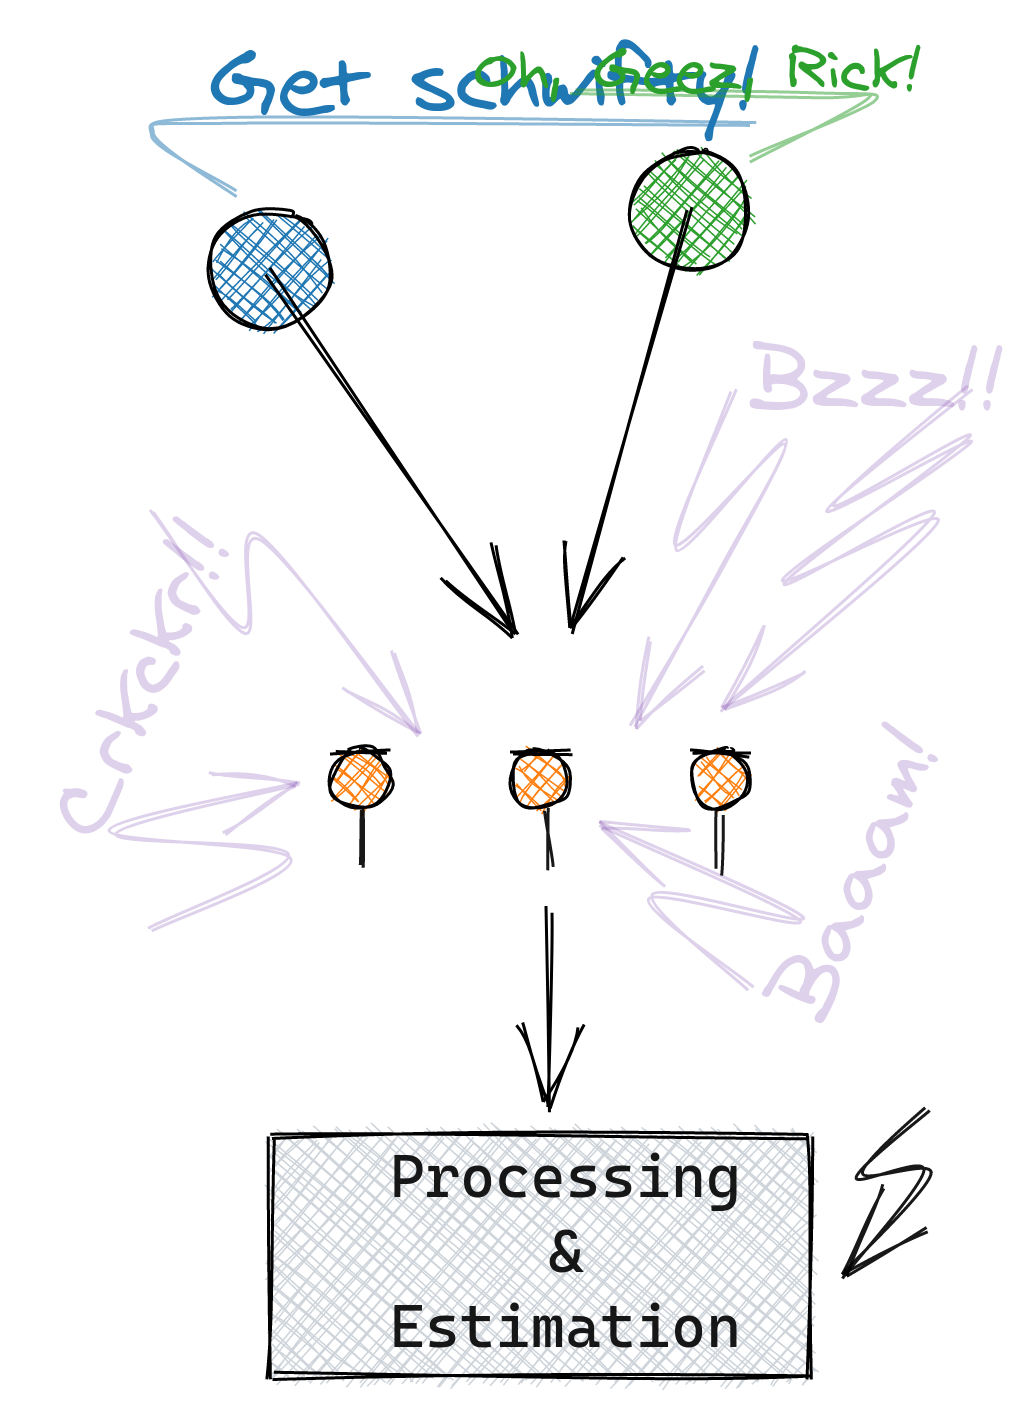
\includegraphics[width=246.25pt,height=335.73pt]{processing/noise.png}};
    % Text Node
    \draw (203.5,100.4) node [anchor=north west][inner sep=0.75pt]  [font=\Large]  {$s_{1}( t)$};
    % Text Node
    \draw (429.5,49.9) node [anchor=north west][inner sep=0.75pt]  [font=\Large]  {$s_{2}( t)$};
    % Text Node
    \draw (455.5,196.9) node [anchor=north west][inner sep=0.75pt]  [font=\Large]  {$\boldsymbol{n}( t)$};
    % Text Node
    \draw (308.5,285.9) node [anchor=north west][inner sep=0.75pt]  [font=\Large]  {$\boldsymbol{x}( t)$};
    % Text Node
    \draw (465.5,327.4) node [anchor=north west][inner sep=0.75pt]  [font=\Large]  {$\boldsymbol{\varepsilon }( t)$};
\end{tikzpicture}
        }
        \captionof{figure}{Graphical representation of the mixing model~\eqref{eq:processing:mixing:mix}:
        $s_2(t)$ is the \textit{interferer},
        $\boldsymbol{n}( t)$ contributes to the \textit{diffuse noise field}, and
        $\boldsymbol{\varepsilon }( t)$ model acquisition and modeling errors.
        }\label{fig:processing:mixing}
}
\newthought{Interfers} identifies the undesired source with properties similar to the target source.
For instance, a concurrent speech source for speech application or concurrent music instrument in case of music.
\\Later, in this thesis the interfer sources will be denoted as additional source indexed by $j > 1$.
\newthought{Noise} collects all the remaining effects, typically nonspeech sources. Moreover we will make a further distinction between the followings.

\newthought{Diffuse Noise Field} describes the background diffuse sources present in the auditory scene, \eg/ car noise, indistinct talking or winds.
It can be recorded or approximated as \AWGN/ with a specific spatial description as described in~\citeonly{habets2007generating}.
% \\In this thesis, it is denoted as $\bsn(t) \sim \calN(0, \cov_{nn})$ where $\cov_{nn} \in \bbR^{I \times I}$ is the noise \textit{spatial covariance matrix}

\newthought{Measurement and Model Noise} accounts for general residual miss- and under-modeling error.
As common is signal processing and information theory, this error term will be modeled as \AWGN/.
\\In this thesis, it will denoted as $\tilde{\varepsilon}_{ij}( t)$ and will be used to model the
approximation of the \RIR/ with the \ISM/ or sensor noise, respectively.

\mynewline
By making the noisy terms explicit, the mixing model in~\cref{eq:processing:mixing:img,eq:processing:mixing:mix} writes:
\begin{align}
    \tilde{\img}_{\idxMic\idxSrc}(t) &=  \kparen{\tilde{\rir}_{\idxMic\idxSrc} \convCont \tilde{\src}_\idxSrc} (t) +  \tilde{\varepsilon}_{ij}(t)\\
    \tilde{\imgs}_\idxSrc(t)         &= \ktranspose{\klist{\tilde{\img}_{1\idxSrc}(t), \dots, \tilde{\img}_{\numMics\idxSrc}(t)}} \nonumber\\
    \tilde{\mics}(t)                 &= \sum_{\idxSrc=1}^{\numSrcs} \tilde{\imgs}_\idxSrc(t) + \tilde{\bsn}( t)
\end{align}

\section{Signal model in the spectral domain}\label{sec:processing:domains}\marginpar{%
    \footnotesize%
    It was introduced by Joseph Fourier in his work on the heat equation~\citeonly{fourier1822theorie}.
    His mathematical tool, named later \textit{Fourier Decomposition},
    aims at approximating any signal by a sum of sine and cosine waves.}%
The frequency, or spectral, representation is probably the most famous signal representation used in signal processing:
Speech and music signals naturally exhibit harmonic and periodic behaviors and
through it are described as combination of sinusoids as function of their frequencies.
% https://tex.stackexchange.com/questions/127375/replicate-the-fourier-transform-time-frequency-domains-correspondence-illustrati

This operation is achieved by the \FTdef/, $\fourierTrans{}:\bbR\kmapsto\bbC$, which projects a continuous-time-domain signal $\tilde{x}$ onto a space spanned by continuous-frequency complex exponentials:
\begin{equation}\label{eq:processing:ft}
    \tilde{X}(f) = (\fourierTrans{\tilde{x}})(f) =
        \int_{-\infty}^{+\infty}
        \tilde{x}(t)
        \cste^{-\csti 2 \pi f t}
        \,\kdiff{t}
    ,
\end{equation}
where $f \in \bbR$ are the \textit{natural frequency} in $\si{\Hz}$ and $\csti$ is the imaginary unit.

\marginpar{

    \centering
    \resizebox{\linewidth}{!}{
        % https://tex.stackexchange.com/questions/127375/replicate-the-fourier-transform-time-frequency-domains-correspondence-illustrati

\begin{tikzpicture} %create tikz picture
\begin{axis}[ %create 3d plot within tikz
    set layers=standard, %use predefined layers
    view={50}{30}, %perspective adjustment
    domain=0:10, %plot limit in time direction
    samples y=1, %samples for frequency direction
    unit vector ratio*=1 2 1, %rescale unit vectors
    hide axis, %do not plot axes
    xtick=\empty, ytick=\empty, ztick=\empty, %no ticks on coordinate axes
    clip=false %let me plot outside the coordinate system
]
    %limit variables
    \def\xmax{100} %limits for curves and layers
    \def\xmin{0}
    \def\ymax{35}
    \def\ymin{5}
    \def\zmax{25}
    \def\zmin{-5}
    \def\xlayer{110} %frequency layer
    \def\sumcurve{0} %sum curve of time signal

    %frequency curves
    \pgfplotsinvokeforeach{1,2,3}{ %for each frequency component
        \draw [on layer=background, lightgray] (axis cs:0,#1,0) -- (axis cs:10,#1,0); %axes
        \addplot3 [on layer=main, darkgray, smooth, samples=200] (x,#1,{1.3*sin(2*#1*x*(157))/(#1*2)}); %plot curves (curves are somewhat arbitrary)

        \xdef\sumcurve{\sumcurve + sin(#1*x*(157))/(#1*2)} %add current curve to sumcurve
    }

    %transparent layers
    \fill[white,opacity=0.7] (\xmin,0,\zmin) -- (\xmin,0,\zmax) -- (\xmax,0,\zmax) -- (\xmax,0,\zmin) -- cycle; %transparent layer in time space
    \fill[white,opacity=0.7] (\xlayer,\ymin,\zmin) -- (\xlayer,\ymin,\zmax) -- (\xlayer,\ymax,\zmax) -- (\xlayer,\ymax,\zmin) -- cycle; % transparent layer for frequency space

    %grid lines
    \pgfplotsinvokeforeach{\xmin,\xmin+5,...,\xmax}{ %create horizontal grid lines (time layer)
        \draw[lightgray,opacity=0.6] (#1,0,\zmin) -- (#1,0,\zmax);
    }
    \pgfplotsinvokeforeach{\ymin,\ymin+2.5,...,\ymax}{ %create horizontal grid lines (frequency layer)
        \draw[lightgray,opacity=0.6] (\xlayer,#1,\zmin) -- (\xlayer,#1,\zmax);
    }
    \pgfplotsinvokeforeach{\zmin,\zmin+5,...,\zmax}{ %create vertical grid lines (both layers)
        \draw[lightgray,opacity=0.6] (\xmin,0,#1) -- (\xmax,0,#1);
        \draw[lightgray,opacity=0.6] (\xlayer,\ymin,#1) -- (\xlayer,\ymax,#1);
    }

    %borders layer
    \draw[midgray] (\xmin,0,\zmin) -- (\xmin,0,\zmax) -- (\xmax,0,\zmax) -- (\xmax,0,\zmin) -- cycle; %time space layer border line
    \draw[midgray] (\xlayer,\ymin,\zmin) -- (\xlayer,\ymin,\zmax) -- (\xlayer,\ymax,\zmax) -- (\xlayer,\ymax,\zmin) -- cycle; %frequency space layer border line

    %sum curve
    \addplot3 [samples=200] (x,0,{\sumcurve+rand/7+0.2*sin(x*400)}); %sum curve time space with added random noise

    % frequency curve
    \addplot3 [name path=f,samples=200,domain=0.5:3.5] (11,x,{rand/30+2*sin((x-0.7)*180)^200*e^(-x/2)-0.3}); %experimentally modified curve with noise

    %create fill under curve
    \addplot3 [name path=ax,draw=none,samples=2,domain=0.5:3.5] (11,x,-0.5); %create fill axis
    \addplot3 [darkgray] fill between [of=f and ax]; %create fill between curve and axis

    %create coordinate axis
    \draw[-{stealth}] (\xmin,0,\zmin-7) -- (\xmax/5.3,0,\zmin-7); %time axis
    \draw[-{stealth}] (\xlayer,\ymin,\zmin-7) -- (\xlayer,\ymin+\ymax/4,\zmin-7); %frequency axis

    %axis labels
    \node[scale=0.7] at (0,0,-21) {Time}; %axis time space
    \node[scale=0.7] at (100,22,-32) {Frequency}; %axis frequency space

\end{axis}
\end{tikzpicture}
    }

    \captionof{figure}{
        A signals resolved into its Fourier series:
        a linear combination of sines and cosines
        represented as peaks in the frequency domain.
    }\label{fig:processing:mixing}
}

A part from providing a space where audio signal reveals their harmonic structures, the Fourier transforms benefits of two fundamental properties:
it is linear and it converts time-convolution into element products.
\\First, linearity allows to write~\cref{eq:processing:mixing:mix} simply as:
\begin{equation}\label{eq:processing:ft:mix}
    \tilde{\mics}( t) = \sum_{\idxSrc=1}^{\numSrcs} \tilde{\imgs}_\idxSrc( t)
    \mathspace\overset{\fourierTrans{}}{\kto}\mathspace
    \tilde{\MICS}( f) = \sum_{\idxSrc=1}^{\numSrcs} \tilde{\IMGS}_\idxSrc( f)
\end{equation}
Secondly, by the \textit{convolution theorem}, the source spatial images in~\cref{eq:processing:mixing:img} writes as:
\begin{equation}\label{eq:processing:conv}
    \tilde{\img}_{\idxMic\idxSrc}( t) =  \kparen{\tilde{\rir}_{\idxMic\idxSrc} \convCont \tilde{\src}_\idxSrc} ( t)
    \mathspace\overset{\fourierTrans{}}{\kto}\mathspace
    \tilde{\IMG}_{\idxMic\idxSrc}( f) =  \tilde{H}_{\idxMic\idxSrc}( f) \tilde{S}_\idxSrc( f)
    .
\end{equation}
As discussed in~\cref{chap:acoustics}, the \FT/ of a \RIR/, \aka/ the \RTFdef/, can be computed exactly in closed-form as
\begin{equation}\label{eq:processing:rir:ft}
    \tilde{H}_{ij}( f) = \sum_{\idxEch=0}^{\numEchs} \absCoeff_{ij}^r \cste^{- \csti 2 \pi f \tau_{ij}^r}
    .
\end{equation}
In practice, the filters $\tilde{h}_{ij}$ are not available in the continuous time domain nor in the continuous frequency domain directly.
They must be estimated from the observation of the discrete-time mixtures $\hat{x}_i[n]$, therefore, after the convolution with a source and the measurement process.
In practice, we don't have access to continuous signal, neither is time and in frequency domain.
Every signal or spectrum the microphones capture are represented by finite- and discrete time signals for which the properties~\eqref{eq:processing:conv} are valid with some precautions.
% That gives rise to the field of digital signal processing.

\subsection{Discrete time and frequency domains}
The spectral representation of a discrete-time signal, $x[n]$ with $n \in \bbZ$, is given by the (forward) \DTFTdef/, $\dtft$:
\begin{equation}\label{eq:processing:dtft}
    \tildeX_{\Fs}(f) = (\dtft{x})(f) =
    \sum_{n = -\infty}^{+\infty}
    x[ n]
    \cste^{-\csti 2 \pi f n / Fs}
    ,
\end{equation}
which is a continuos function of $f$ with period $\Fs$.
Notice that the term \underline{discrete-time} refers to the fact that the transform operates on discrete signal.
When this samples are uniformly spaced at rate $\Fs$, it produces a function of continuous frequency that is a periodic summation of the continuous Fourier transform of the original continuous function.
Under certain theoretical conditions, described by the \textit{sampling theorem}, both the original continuous signal $\tildex$ and its sampled version $\hatx$ can be recovered perfectly from the \DTFT/.
The \DTFT/ itself is a continuous function of frequency which require infinite discrete value to be computed.
For these two reason, it is not accessible in practice or computed in the digital domain.
Therefore the following representation is used instead.

The spectral representation of a discrete- and finite-time signal $\hat{x}_N$ is given by its (forward) \DFTdef/
\sidenote{
    This can be intrepreded as the projection onto the space spanned by a finite number of complex exponentials.
},
$\discreteFT{}:\bbR^N\kmapsto\bbC$:
\begin{equation}\label{eq:processing:dft}
    \hat{X}_F[ k] = (\discreteFT{\hat{x}_N})[k] =
    \sum_{n = 0}^{N - 1}
    \hat{x}_N[ n]
    \cste^{-\csti2\pi k n / F}
    .
\end{equation}
where $k \in \kintervcc{0}{F - 1}$ is the discrete \textit{frequency bin} and $F$ is the total number of bins.
Again we use the subscript $F$ and the brackets $[k]$ to stress the finite and discrete frequency support of the $\DFT/$.
\\The natural frequency $f_k$ in $\si{\Hz}$ corresponding to the $k$-th frequency bin can be computed as
\begin{equation}\label{eq:processing:fk}
    f_k = \frac{k}{F}\Fs
    .
\end{equation}

\subsection{The DFT as approximation of the FT}\label{subsec:processing:ftapprox}
An important application of the \DFT/ is to approximate numerically the \FT/.
As mentioned at the beginning of the chapter, with the discretisation process the continuous signal is periodically sampled, low-passed and finally truncated.
It can be proved that sampling in the time domain corresponds to limiting the signal bandwidth and periodizing the spectrum.
\\By assuming sampling at rate $\Fs$, in the continuos-frequency domain the spectrum $\tilde{X}(f)$ is repeated every internals of size $\Fs\,\si{\Hz}$ .
By further assuming that the signal undergoes an ideal low-pass filter, no spectral leakage is presents between each repetition.
\\So far, the sampled time domain signal, $\hat{x}[n]$, is mapped to the continuous frequency domain $\tilde{X}(f)$.
This particular case of the \FT/ is called \DTFTdef/ and it is denote with $\tilde{X}_{\Fs}[ k]$.
\begin{equation}\label{eq:processing:ft2dtft}
    \begin{aligned}
        \tilde{X}(f) =
        \int_{-\infty}^{+\infty}
        \tilde{x}(t)
        \cste^{-\csti 2 \pi f t}
        \,\kdiff{t}
        \quad \rightarrow \quad
        \tilde{X}_{\Fs}( f) =
        \sum_{n = -\infty}^{\infty}
        \hat{x}[ n]
        \cste^{-\csti2\pi f \frac{n}{\Fs}}
    \end{aligned}
    .
\end{equation}
Here the continuous integral the \FT/ is approximated by Riemann sum over the discrete points $n \in \Z$:
To be more rigorous, when computing a Riemann sum approximation, the length of the discretisation interval multiply the summation.
In our application, this quantity always set to $\Fs$ and for readability reason such term is dropped.
\\The quality of this approximation \wrt/ the original continuous spectrum is regulated by the choice of $\Fs$: the higher $\Fs$, the better the approximation.
The upper bound to the possible value $\Fs$ is the results known as the Nyquist–Shannon's sampling theorem.

\mynewline
Furthermore, we consider only the finite sequence $\hat{x}_N$ consisting of $N$ samples.
This would reduce the summation ranges the right part of~\cref{eq:processing:ft2dtft}.
Instead, we can keep the infinite summation by multiplying the sampled signal by a discrete-time window function $\hat{w}$ selecting the non-zero porting of $\hat{x}$, $\hat{x}_N[n] = \hat{w}[n]\hat{x}[n]$.
By the \textit{convolution theorem}, the multiplication in the time domain translates in a convolution between the corresponding spectra.
As a consequence, the spectrum of the truncated signal is distorted by the spectrum of the window function.
In math,
\begin{equation}\label{eq:processing:ft2dtft}
    \tilde{X}_N(f) =
    \sum_{n=0}^{N-1}
    \hat{x}_N[n]
    \cste^{-\csti2\pi f \frac{n}{\Fs}}
    \quad \leftrightarrow \quad
    \tilde{X}_{\Fs}( f) =
    \sum_{n = -\infty}^{\infty}
    \hat{x}[ n] \hat{w}[ n]
    \cste^{-\csti2\pi f \frac{n}{\Fs}}
    .
\end{equation}
By the convolution theorem, we have that
\begin{equation}
    \hat{x}_N[n] = \hat{x}[ n] \hat{w}[ n]
    \quad \leftrightarrow \quad
    \tilde{X}_{N}(f) = (\tilde{X}_{\Fs} \convCont \tilde{W}_{\Fs})(f)
\end{equation}
where $\tilde{W}_{\Fs}$ is the \DTFT/ of the sampled window function $\hat{w}[n]$.
\\Assuming the window function to be an ideal door function\sidenote{door function here}, its \DTFT/ is a ideal low-pass filter, which acts on the original spectrum as a smoothing function.
As a consequence, the quality of this approximation is then based on the spectral leakage of the chosen window function, $w[n]$.
As a rule of thumb, here the longer the segment, the better the approximation%
\sidenote{When short excerpt are considered instead (\eg/ in case of the \STFTdef/), particular types of window function are used but their analysis are out of the scope of this thesis.}

\mynewline
Finally, we cannot access the \DTFT/ directly because that involves an infinite number of frequencies $f \in \R$.
Therefore, taking $F$ uniformly-spaced frequency $f_k\in\R$ as in~\cref{eq:processing:fk}, we finally obtain the \DFT/ as in~\cref{eq:processing:dft}, that is
\begin{equation}
    \tilde{X}_N(f_k) =
    \sum_{n=0}^{N-1}
    \hat{x}_N[n]
    \cste^{-\csti2\pi f \frac{n}{\Fs}}
    \quad \leftrightarrow \quad
    \hat{X}_F[k] =
    \sum_{n=0}^{N-1}
    \hat{x}_N[n]
    \cste^{-\csti2\pi k n / F}
    .
\end{equation}
Notice that the $\Fs$ term disappeared in the right part of the equation above as it cancels out when using~\cref{eq:processing:fk}.
By increasing $F$, we can sample more densely $\hat{X}_F[k]$ which leads to a better approximation to $\tilde{X}_N$.
However this does not eliminates the distortion of the previous steps, due to $\tilde{W}_{\Fs}$.

\mynewline
Again, we sampled a domain. Thus, according to the defined sampling process, this involve using a ideal low-pass filter.
This filter acts now on the discrete spectrum, smoothing it and limiting the support of its transformation in the dual domain.
Therefore, the inverse \DFT/ of $\hat{X}_F[k]$ is not properly $\hat{x}_N[n]$, but its periodic version repeated every $F$ samples.
In fact, sampling in one of the two domain is equivalent to a periodization in the other domain while truncating lead to convolving with a window function.
Moreover, the chain of operation (sampling in time and truncation in time and sampling in frequencies) are valid in both way.
Thus one can arbitrarily first sample and truncate frequency domain and finally sample in time.
The only difference is in the interpretation of the windowing function, which in one case smooth the spectrum and in the other smooth the signal.
All this relation and approximation that connects the \FT/ to the \DFT/ are well explained in explanatory material presented in~\sidenote{\url{https://krasjet.com/rnd.wlk/poisson.pdf}}.

% Through the use of microphones and computers, our window into the continuous physical world of acoustics is narrow and discrete, both it time and in frequency.

\subsection{Signal model in the discrete Fourier domain}\label{sec:processing:fouriermodel}
Conscious of the above approximations, we can now rewrite our signal model for the discrete case.
Hereafter we will always consider finite-length sequences and the index $N$ will be dropped to lighten the notation.
\\The \DFT/ is linear, so the discrete version of \cref{eq:processing:ft:mix} becomes
\begin{equation}\label{eq:processing:dft:mix}
    \hat{\mics}[ n] = \sum_{\idxSrc=1}^{\numSrcs} \hat{\imgs}_\idxSrc[ n]
    \mathspace\overset{\discreteFT}{\kto}\mathspace
    \hat{\MICS}[ k] = \sum_{\idxSrc=1}^{\numSrcs} \hat{\IMGS}_\idxSrc[ k]
\end{equation}
Secondly, by using na\"ively the discrete convolution theorem, one could translate \cref{eq:processing:mixing:img} as
\begin{equation}\label{eq:processing:discreteModel}
    \hat{\img}_{ij}[n] = (\hat{\rir}_{ij} \convDis \hat{\src})[n]
    \mathspace\overset{\discreteFT{}}{\kto}\mathspace
    \hat{C}_{ij}[k] = \hat{H}_{ij}[k] \hat{S}[k]
    ,
\end{equation}
where $\convDis$ is the finite-time linear convolution operator\sidenote{
    The finite-time linear convolution for two vectors $\hatu\in\bbR^L$ and $\hatv\in\bbR^D$ is
    \\$(\hatu \convDis \hatv)[n] = \sum_{l=0}^{L-1} \hatu[l] \hatv[L-1+n-j]$ for $n = 0, \cdots, D-L$
    .
}.
\\The filter $\hat{H}_{ij}[k]$ is the \DFT/ of the room impulse response.
As mentioned in the~\cref{subsec:processing:ftapprox}, this just approximates the \RTF/ of~\cref{eq:processing:rtf}.
Thus we can write,
\begin{equation}\label{eq:processing:discreteModel:rir}
    \hat{H}_{ij}[ k] \approx \sum_{\idxEch=0}^{\numEchs}
                \frac{\absCoeff_{ij}^r}{4 \pi \speedOfSound \tau_{ij}^r}
                \cste^{- \csti 2 \pi k \Fs \tau_{ij}^r / F}
    .
\end{equation}

\mynewline
Although used in practice, the model~\eqref{eq:processing:discreteModel} makes use of other approximations that are worth presenting.
In particular, the work by~\citeonly{tukuljac2018mulan} properly discuss them in the context of the echo estimation problem.
The paper mention three approximations, which are depicted in the following diagram.

\begin{figure}[!h]
    \begin{fullwidth}
    \centering
    

\tikzset{every picture/.style={line width=0.75pt}} %set default line width to 0.75pt

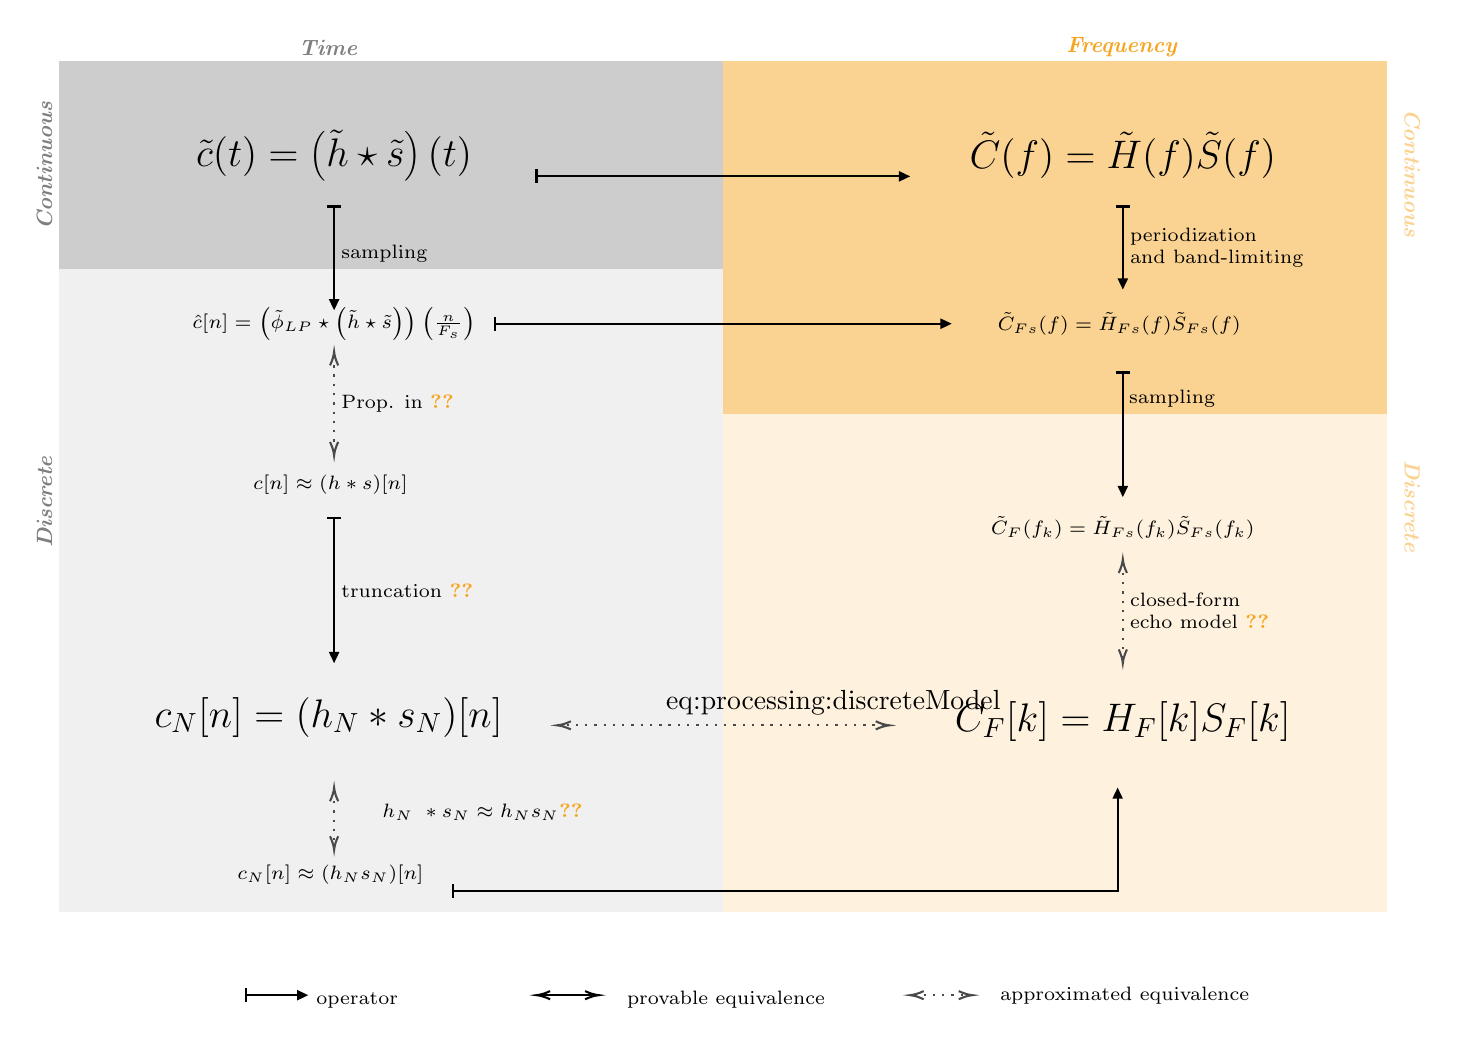
\begin{tikzpicture}[x=0.75pt,y=0.75pt,yscale=-1,xscale=1]
%uncomment if require: \path (0,510); %set diagram left start at 0, and has height of 510

%Shape: Rectangle [id:dp4992481295668366]
\draw  [draw opacity=0][fill={rgb, 255:red, 245; green, 166; blue, 35 }  ,fill opacity=0.15 ] (350,200) -- (670,200) -- (670,440) -- (350,440) -- cycle ;
%Shape: Rectangle [id:dp43040154350776516]
\draw  [draw opacity=0][fill={rgb, 255:red, 155; green, 155; blue, 155 }  ,fill opacity=0.15 ] (30,130) -- (350,130) -- (350,440) -- (30,440) -- cycle ;
%Shape: Rectangle [id:dp8042559757750585]
\draw  [draw opacity=0] (50,260) -- (650,260) -- (650,300) -- (50,300) -- cycle ;
%Shape: Rectangle [id:dp20306390916355643]
\draw  [draw opacity=0][fill={rgb, 255:red, 155; green, 155; blue, 155 }  ,fill opacity=0.5 ] (30,30) -- (350,30) -- (350,130) -- (30,130) -- cycle ;
%Shape: Rectangle [id:dp44418021353360915]
\draw  [draw opacity=0][fill={rgb, 255:red, 245; green, 166; blue, 35 }  ,fill opacity=0.5 ] (350,30) -- (670,30) -- (670,200) -- (350,200) -- cycle ;
%Straight Lines [id:da7171827150721688]
\draw    (162.5,100) -- (162.5,147) ;
\draw [shift={(162.5,150)}, rotate = 270] [fill={rgb, 255:red, 0; green, 0; blue, 0 }  ][line width=0.08]  [draw opacity=0] (5.36,-2.57) -- (0,0) -- (5.36,2.57) -- cycle    ;
\draw [shift={(162.5,100)}, rotate = 270] [color={rgb, 255:red, 0; green, 0; blue, 0 }  ][line width=0.75]    (0,3.35) -- (0,-3.35)   ;
%Straight Lines [id:da6469277791434447]
\draw [color={rgb, 255:red, 74; green, 74; blue, 74 }  ,draw opacity=1 ] [dash pattern={on 0.84pt off 2.51pt}]  (162.5,172) -- (162.5,218) ;
\draw [shift={(162.5,220)}, rotate = 270] [color={rgb, 255:red, 74; green, 74; blue, 74 }  ,draw opacity=1 ][line width=0.75]    (6.56,-1.97) .. controls (4.17,-0.84) and (1.99,-0.18) .. (0,0) .. controls (1.99,0.18) and (4.17,0.84) .. (6.56,1.97)   ;
\draw [shift={(162.5,170)}, rotate = 90] [color={rgb, 255:red, 74; green, 74; blue, 74 }  ,draw opacity=1 ][line width=0.75]    (6.56,-1.97) .. controls (4.17,-0.84) and (1.99,-0.18) .. (0,0) .. controls (1.99,0.18) and (4.17,0.84) .. (6.56,1.97)   ;
%Straight Lines [id:da7251536612909463]
\draw [color={rgb, 255:red, 74; green, 74; blue, 74 }  ,draw opacity=1 ] [dash pattern={on 0.84pt off 2.51pt}]  (542.5,272) -- (542.5,318) ;
\draw [shift={(542.5,320)}, rotate = 270] [color={rgb, 255:red, 74; green, 74; blue, 74 }  ,draw opacity=1 ][line width=0.75]    (6.56,-1.97) .. controls (4.17,-0.84) and (1.99,-0.18) .. (0,0) .. controls (1.99,0.18) and (4.17,0.84) .. (6.56,1.97)   ;
\draw [shift={(542.5,270)}, rotate = 90] [color={rgb, 255:red, 74; green, 74; blue, 74 }  ,draw opacity=1 ][line width=0.75]    (6.56,-1.97) .. controls (4.17,-0.84) and (1.99,-0.18) .. (0,0) .. controls (1.99,0.18) and (4.17,0.84) .. (6.56,1.97)   ;
%Straight Lines [id:da5947956265023664]
\draw    (542.5,100) -- (542.5,137) ;
\draw [shift={(542.5,140)}, rotate = 270] [fill={rgb, 255:red, 0; green, 0; blue, 0 }  ][line width=0.08]  [draw opacity=0] (5.36,-2.57) -- (0,0) -- (5.36,2.57) -- cycle    ;
\draw [shift={(542.5,100)}, rotate = 270] [color={rgb, 255:red, 0; green, 0; blue, 0 }  ][line width=0.75]    (0,3.35) -- (0,-3.35)   ;
%Straight Lines [id:da19099903743367053]
\draw    (260,85.5) -- (437,85.5) ;
\draw [shift={(440,85.5)}, rotate = 180] [fill={rgb, 255:red, 0; green, 0; blue, 0 }  ][line width=0.08]  [draw opacity=0] (5.36,-2.57) -- (0,0) -- (5.36,2.57) -- cycle    ;
\draw [shift={(260,85.5)}, rotate = 180] [color={rgb, 255:red, 0; green, 0; blue, 0 }  ][line width=0.75]    (0,3.35) -- (0,-3.35)   ;
%Straight Lines [id:da7382102198689917]
\draw    (120,480) -- (147,480) ;
\draw [shift={(150,480)}, rotate = 180] [fill={rgb, 255:red, 0; green, 0; blue, 0 }  ][line width=0.08]  [draw opacity=0] (5.36,-2.57) -- (0,0) -- (5.36,2.57) -- cycle    ;
\draw [shift={(120,480)}, rotate = 180] [color={rgb, 255:red, 0; green, 0; blue, 0 }  ][line width=0.75]    (0,3.35) -- (0,-3.35)   ;
%Straight Lines [id:da4522721370395596]
\draw [color={rgb, 255:red, 74; green, 74; blue, 74 }  ,draw opacity=1 ] [dash pattern={on 0.84pt off 2.51pt}]  (442,480) -- (468,480) ;
\draw [shift={(470,480)}, rotate = 180] [color={rgb, 255:red, 74; green, 74; blue, 74 }  ,draw opacity=1 ][line width=0.75]    (6.56,-1.97) .. controls (4.17,-0.84) and (1.99,-0.18) .. (0,0) .. controls (1.99,0.18) and (4.17,0.84) .. (6.56,1.97)   ;
\draw [shift={(440,480)}, rotate = 0] [color={rgb, 255:red, 74; green, 74; blue, 74 }  ,draw opacity=1 ][line width=0.75]    (6.56,-1.97) .. controls (4.17,-0.84) and (1.99,-0.18) .. (0,0) .. controls (1.99,0.18) and (4.17,0.84) .. (6.56,1.97)   ;
%Straight Lines [id:da6235625122330559]
\draw    (262,480) -- (288,480) ;
\draw [shift={(290,480)}, rotate = 180] [color={rgb, 255:red, 0; green, 0; blue, 0 }  ][line width=0.75]    (6.56,-1.97) .. controls (4.17,-0.84) and (1.99,-0.18) .. (0,0) .. controls (1.99,0.18) and (4.17,0.84) .. (6.56,1.97)   ;
\draw [shift={(260,480)}, rotate = 0] [color={rgb, 255:red, 0; green, 0; blue, 0 }  ][line width=0.75]    (6.56,-1.97) .. controls (4.17,-0.84) and (1.99,-0.18) .. (0,0) .. controls (1.99,0.18) and (4.17,0.84) .. (6.56,1.97)   ;
%Straight Lines [id:da19953036714140948]
\draw    (162.5,250) -- (162.5,317) ;
\draw [shift={(162.5,320)}, rotate = 270] [fill={rgb, 255:red, 0; green, 0; blue, 0 }  ][line width=0.08]  [draw opacity=0] (5.36,-2.57) -- (0,0) -- (5.36,2.57) -- cycle    ;
\draw [shift={(162.5,250)}, rotate = 270] [color={rgb, 255:red, 0; green, 0; blue, 0 }  ][line width=0.75]    (0,3.35) -- (0,-3.35)   ;
%Straight Lines [id:da6866901501479744]
\draw    (240,156.5) -- (457,156.5) ;
\draw [shift={(460,156.5)}, rotate = 180] [fill={rgb, 255:red, 0; green, 0; blue, 0 }  ][line width=0.08]  [draw opacity=0] (5.36,-2.57) -- (0,0) -- (5.36,2.57) -- cycle    ;
\draw [shift={(240,156.5)}, rotate = 180] [color={rgb, 255:red, 0; green, 0; blue, 0 }  ][line width=0.75]    (0,3.35) -- (0,-3.35)   ;
%Straight Lines [id:da07357493408339133]
\draw    (542.5,180) -- (542.5,237) ;
\draw [shift={(542.5,240)}, rotate = 270] [fill={rgb, 255:red, 0; green, 0; blue, 0 }  ][line width=0.08]  [draw opacity=0] (5.36,-2.57) -- (0,0) -- (5.36,2.57) -- cycle    ;
\draw [shift={(542.5,180)}, rotate = 270] [color={rgb, 255:red, 0; green, 0; blue, 0 }  ][line width=0.75]    (0,3.35) -- (0,-3.35)   ;
%Straight Lines [id:da2666798410307448]
\draw [color={rgb, 255:red, 74; green, 74; blue, 74 }  ,draw opacity=1 ] [dash pattern={on 0.84pt off 2.51pt}]  (162.5,382) -- (162.5,408) ;
\draw [shift={(162.5,410)}, rotate = 270] [color={rgb, 255:red, 74; green, 74; blue, 74 }  ,draw opacity=1 ][line width=0.75]    (6.56,-1.97) .. controls (4.17,-0.84) and (1.99,-0.18) .. (0,0) .. controls (1.99,0.18) and (4.17,0.84) .. (6.56,1.97)   ;
\draw [shift={(162.5,380)}, rotate = 90] [color={rgb, 255:red, 74; green, 74; blue, 74 }  ,draw opacity=1 ][line width=0.75]    (6.56,-1.97) .. controls (4.17,-0.84) and (1.99,-0.18) .. (0,0) .. controls (1.99,0.18) and (4.17,0.84) .. (6.56,1.97)   ;
%Straight Lines [id:da25295598066707925]
\draw    (220,430) -- (540,430) -- (540,383) ;
\draw [shift={(540,380)}, rotate = 450] [fill={rgb, 255:red, 0; green, 0; blue, 0 }  ][line width=0.08]  [draw opacity=0] (5.36,-2.57) -- (0,0) -- (5.36,2.57) -- cycle    ;
\draw [shift={(220,430)}, rotate = 180] [color={rgb, 255:red, 0; green, 0; blue, 0 }  ][line width=0.75]    (0,3.35) -- (0,-3.35)   ;
%Straight Lines [id:da6393966024560223]
\draw [color={rgb, 255:red, 74; green, 74; blue, 74 }  ,draw opacity=1 ] [dash pattern={on 0.84pt off 2.51pt}]  (270,350) -- (427,350) ;
\draw [shift={(430,350)}, rotate = 180] [color={rgb, 255:red, 74; green, 74; blue, 74 }  ,draw opacity=1 ][line width=0.75]    (6.56,-1.97) .. controls (4.17,-0.84) and (1.99,-0.18) .. (0,0) .. controls (1.99,0.18) and (4.17,0.84) .. (6.56,1.97)   ;
\draw [shift={(270,350)}, rotate = 0] [color={rgb, 255:red, 74; green, 74; blue, 74 }  ,draw opacity=1 ][line width=0.75]    (6.56,-1.97) .. controls (4.17,-0.84) and (1.99,-0.18) .. (0,0) .. controls (1.99,0.18) and (4.17,0.84) .. (6.56,1.97)   ;
% Text Node
\draw (162.5,75.5) node  [font=\Large]  {$\tilde{c}( t) =\left(\tilde{h} \star \tilde{s}\right)( t)$};
% Text Node
\draw (542.5,75.5) node  [font=\Large]  {$\tilde{C}( f) =\tilde{H}( f)\tilde{S}( f)$};
% Text Node
\draw (164.5,195) node [anchor=west] [inner sep=0.75pt]  [font=\scriptsize] [align=left] {\textcolor[rgb]{0,0,0}{Prop. in }\textcolor[rgb]{0.96,0.65,0.14}{\ref{it:processing:dft:approx1}}};
% Text Node
\draw (164.5,285) node [anchor=west] [inner sep=0.75pt]  [font=\scriptsize] [align=left] {truncation \textcolor[rgb]{0.96,0.65,0.14}{\ref{it:processing:dft:approx2}}};
% Text Node
\draw (163,346) node  [font=\Large]  {$c_{N}[ n] =( h_{N} \ast s_{N})[ n] \ $};
% Text Node
\draw  [draw opacity=0]  (482.5,143.5) -- (602.5,143.5) -- (602.5,169.5) -- (482.5,169.5) -- cycle  ;
\draw (542.5,156.5) node  [font=\scriptsize]  {$\tilde{C}_{Fs}( f) =\tilde{H}_{Fs}( f)\tilde{S}_{Fs}( f) \ $};
% Text Node
\draw  [draw opacity=0]  (89,139.5) -- (236,139.5) -- (236,173.5) -- (89,173.5) -- cycle  ;
\draw (162.5,156.5) node  [font=\scriptsize]  {$\ \hat{c}[ n] =\left(\tilde{\phi }_{LP} \star \left(\tilde{h} \star \tilde{s}\right)\right)\left(\frac{n}{F_{s}}\right) \ $};
% Text Node
\draw (542.5,348.25) node  [font=\Large]  {$C_{F}[ k] =H_{F}[ k] S_{F}[ k]$};
% Text Node
\draw  [draw opacity=0]  (119,225) -- (206,225) -- (206,243) -- (119,243) -- cycle  ;
\draw (162.5,234) node  [font=\scriptsize]  {$c[ n] \approx ( h\ast s)[ n] \ $};
% Text Node
\draw (160,23.5) node  [font=\footnotesize,color={rgb, 255:red, 0; green, 0; blue, 0 }  ,opacity=0.5 ] [align=left] {\textit{\textbf{Time}}};
% Text Node
\draw (542.5,23) node  [font=\footnotesize,color={rgb, 255:red, 245; green, 166; blue, 35 }  ,opacity=1 ] [align=left] {\textit{\textbf{Frequency}}};
% Text Node
\draw (23,80) node  [font=\footnotesize,color={rgb, 255:red, 0; green, 0; blue, 0 }  ,opacity=0.5 ,rotate=-270] [align=left] {\textit{\textbf{Continuous}}};
% Text Node
\draw (23,242) node  [font=\footnotesize,color={rgb, 255:red, 0; green, 0; blue, 0 }  ,opacity=0.5 ,rotate=-270] [align=left] {\begin{minipage}[lt]{34.192644pt}\setlength\topsep{0pt}
\begin{center}
\textit{\textbf{Discrete}}
\end{center}

\end{minipage}};
% Text Node
\draw (326,58.4) node [anchor=north west][inner sep=0.75pt]  [font=\Large]  {$\fourierTrans{}$};
% Text Node
\draw (173.6,482.35) node  [font=\scriptsize] [align=left] {operator};
% Text Node
\draw (351.31,482.35) node  [font=\scriptsize] [align=left] {provable equivalence};
% Text Node
\draw (543.38,480.35) node  [font=\scriptsize] [align=left] {approximated equivalence};
% Text Node
\draw (164.5,122.5) node [anchor=west] [inner sep=0.75pt]  [font=\scriptsize] [align=left] {sampling};
% Text Node
\draw (544.5,120) node [anchor=west] [inner sep=0.75pt]  [font=\scriptsize] [align=left] {periodization \\and band-limiting};
% Text Node
\draw (326,129.4) node [anchor=north west][inner sep=0.75pt]  [font=\Large]  {$\dtft$};
% Text Node
\draw (544,192.5) node [anchor=west] [inner sep=0.75pt]  [font=\scriptsize] [align=left] {sampling};
% Text Node
\draw  [draw opacity=0]  (478.5,242) -- (606.5,242) -- (606.5,268) -- (478.5,268) -- cycle  ;
\draw (542.5,255) node  [font=\scriptsize]  {$\tilde{C}_{F}( f_{k}) =\tilde{H}_{Fs}( f_{k})\tilde{S}_{Fs}( f_{k})$};
% Text Node
\draw (682,84) node  [font=\footnotesize,color={rgb, 255:red, 0; green, 0; blue, 0 }  ,opacity=0.5 ,rotate=-90] [align=left] {\textit{\textbf{\textcolor[rgb]{0.96,0.65,0.14}{Continuous}}}};
% Text Node
\draw (682,244.5) node  [font=\footnotesize,color={rgb, 255:red, 0; green, 0; blue, 0 }  ,opacity=0.5 ,rotate=-90] [align=left] {\begin{minipage}[lt]{34.192644pt}\setlength\topsep{0pt}
\begin{center}
\textit{\textbf{\textcolor[rgb]{0.96,0.65,0.14}{Discrete}}}
\end{center}

\end{minipage}};
% Text Node
\draw (162.5,422.14) node  [font=\scriptsize]  {$c_{N}[ n] \approx ( h_{N} \circledast s_{N})[ n] \ $};
% Text Node
\draw (234,392) node  [font=\scriptsize] [align=left] {\textcolor[rgb]{0,0,0}{ }\textcolor[rgb]{0,0,0}{$\displaystyle h_{N} \ \ast s_{N} \approx h_{N} \circledast s_{N}$}\textcolor[rgb]{0,0,0}{ }\textcolor[rgb]{0.96,0.65,0.14}{\ref{it:processing:dft:approx2}}};
% Text Node
\draw (326,403.4) node [anchor=north west][inner sep=0.75pt]  [font=\Large]  {$\discreteFT{}$};
% Text Node
\draw (544.5,295) node [anchor=west] [inner sep=0.75pt]  [font=\scriptsize] [align=left] {closed-form \\echo model \textcolor[rgb]{0.96,0.65,0.14}{\ref{it:processing:dft:approx3}}};
% Text Node
\draw (321,331.4) node [anchor=north west][inner sep=0.75pt]  [font=\normalsize]  {\cref{eq:processing:discreteModel}};


\end{tikzpicture}

    \end{fullwidth}
\end{figure}

The diagram shows a chain of operators (sampling and transforms) with provable and approximated equivalences that lead to~\cref{eq:processing:discreteModel} used in practice.
In order,
\begin{enumerate}[label=(\roman*)]
    \item\label{it:processing:dft:approx1}
    In~\citeonly{van2001gaussian}, the Proposition 2 shows that if the signal $\tilde{\src}(t)$ is band-limited by $\Fs$,
    then sampling the continuous convolution is exactly equivalent to \textit{linearly convolving} the infinite discrete signal $\hat{\src}[n]$ and the discrete and low-passed version of the filter.
    While the source signal is band-limited by nature, $\tilde{h}(t)$ is not (in fact the \RIR/ is modeled as a summation of spikes, which has infinite spectrum).
    Thus, the first approximation~\ref{it:processing:dft:approx1} considers $\hat{h}[n] \approx (\lowpassfilter \convDis \tilde{h})[n]$, in words
    we assume that the filter is band-limited by $\pm \sfrac{\Fs}{2}$.
    \\\citeauthor{tukuljac2018mulan} made an important observation here:
    even if infinite number of samples are available, after the measurement process, the discrete-time filter $\hat{\rir}[n]$ consists of infinite-length decimated combinations of sinc functions.
    \\In the context of this thesis, this observation tell us that even in ideal conditions, that is without noise, possibly knowing the transmitted signal, and processing infinitely
    many samples, the exact estimation of the echo properties of the \RIR/ is challenging task itself. This is a fundamental difference between \RIR/ estimation and estimating the
    time of arrivals of the early echoes.
    \\Note, for instance, that we wrote the echo model only in the continuous-time domain or with its closed-form form discrete frequencies.
    The discrete-time domain was avoided on purpose since the echoes' arrival time are naturally off the sampling grid, namely not integer multiple $\Fs$.

    \item\label{it:processing:dft:approx2}
    The discrete-time convolution theorem applies to the \textit{circular convolution}, which can be approximated by the \textit{linear convolution}
    that is $(\hath \circledast \hats)[n] \approx (\hath \convDis \hats)[n]$.
    This second approximation is reasonably good when many samples are available and when one of the two signals is periodic, which
    are typical cases for audio signals.

    \item\label{it:processing:dft:approx3}
    The third approximation regards the closed-form of $h_{ij}(f)$ of~\cref{eq:processing:discreteModel:rir} which
    would require infinitely many samples and unlimited frequency support to be computed\sidenote{This formula would results from the \DTFTdef/ of $\tilde{\rir}_{ij}(t)$}.
\end{enumerate}

Nevertheless, it is important to notice that approximations \ref{it:processing:dft:approx2} and \ref{it:processing:dft:approx3} become arbitrarily precise as the number of samples $N$ grows to infinity.

\mynewline
While the raw audio signal encodes the amplitude of a sound as a function of time,
its spectrum represents it as a function of frequency.
In order to jointly account for both temporal and spectral characteristic, joint time-frequency representations are used.

\subsection{Time-Frequency domain representation}\label{subsec:processing:stft}
\TFdef/ representations aim to jointly describe the signal in the time and frequency domains.
Instead of considering the entire signal, the main idea is to consider only a small section of the signal.
To this end, one fixes a so-called \textit{window} function, $\hatw_N[n]$, which is nonzero for only a period of time $\winsize$ shorter than the entire signal length, $\winsize \ll N$.
This function iteratively shifts and multiplies the original signal, producing consecutive \textit{frames}.
Finally, the frequency information are extracted independently from each frame.
The choice of a window function $w[n]$ depends on the application since its contribution reflects in the \TF/ representation together with the
one of the signal.

\newthought{The discrete \STFT/}\marginpar{\footnotesize%
The \STFT/ was introduced by Dennis Gabor in the 1946, the person behind Holography and Gaborlets.
}
is the most commonly used \TF/-representation in audio signal processing.
This representation encodes the time-varying spectra into a matrix $X[k,l] \in \bbC^{F,T}$ with frequency index $k$ and time frame index $l$.
More formally, the process to compute the complex \STFT/ coefficients is given by
\begin{equation}\label{eq:processing:stft}
    X[k, l]  = \sum_{n=0}^{\winsize-1} w[n] x[n + l \hopsize] \cste^{- \csti 2 \pi k n / F} \mathspace\in\bbC
\end{equation}
where $\winsize$ is the window length and $\hopsize$ is the \textit{hop size} which specifies how much the window needs to be shifted across the signal.
Equivalently, \cref{eq:processing:stft} can be expressed as \DFT/s of windowed frames, $X[k, l] = \discreteFT{\hatx[n,l]}$ where $\hatx[n,l] = \hatx[n + l \hopsize] \hatw[n]$.

Since each \STFT/ coefficient $x[k, l]$ lives in the complex space $\bbC$, the squared magnitude of the \STFT/, $\powerOf{\hatX[k,l]}$ is
commonly used for visualization and for processing
\marginpar{
    \centering
    \footnotesize
    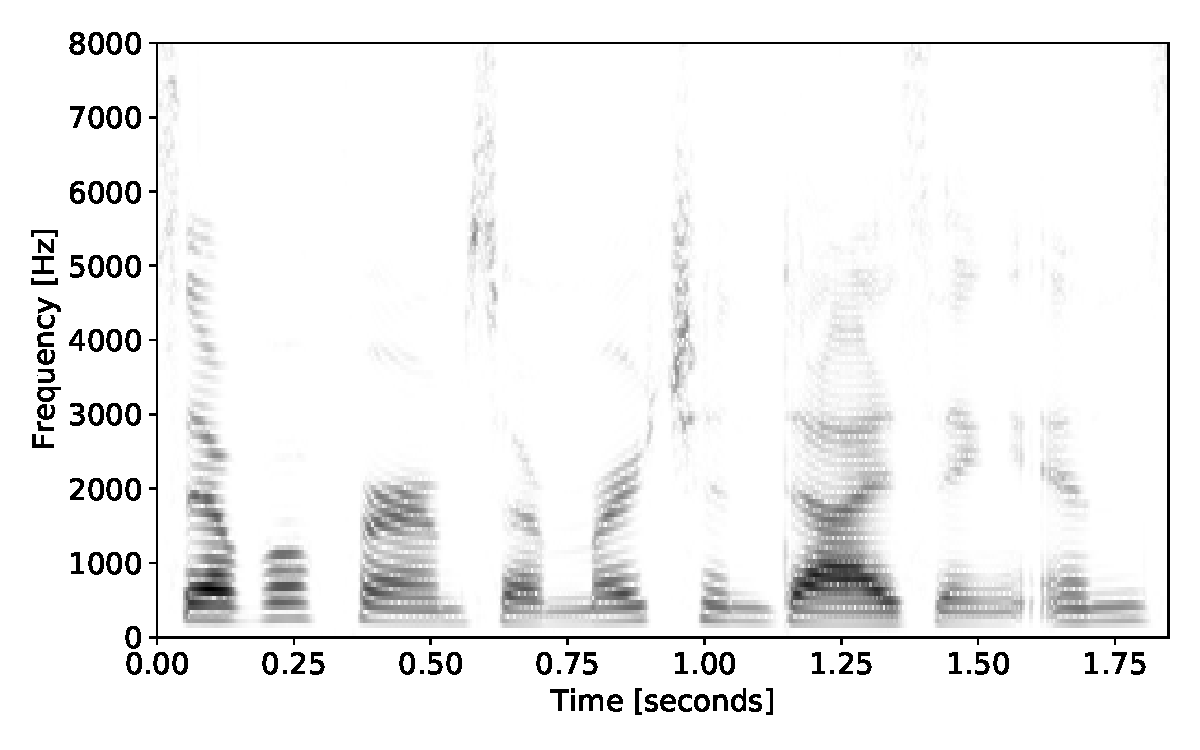
\includegraphics[width=\linewidth]{processing/py-speech_spectrogram.pdf}
    \captionof{figure}{STFT spectrogram of an example speech signal. Higher energies are illustrated with darker colors.}
    \label{fig:processing:spectrogram}
}%\sidenote{The phase in some application is completely ignored because of difficult interpretation or commonly considered less informative with respect to the sound magnitude}.
The resulting two-dimensional representation is called (log) \textit{spectrogram}.
It can be visualized by means of a two-dimensional image, whose axes represent time frames and frequency bins.
In this image, the (log) value $\powerOf{\hatX[k,l]}$ is represented by the intensity or color in the image at the coordinate $[k,l]$.
Throughout this works both estimation and processing will be typically conducted in the \STFT/ domain, unless specified.
This is a common approach in the audio signal processing community, but it is not the only one:
many algorithm are designed directly in the time domain or in alternatives \TF/ representation, \eg/ Mel-Scale, Filter-Banks, or the quadratic STFT transform used in~\cref{ch:brioche}.

\marginpar{%
    \vspace{-4cm}
    \footnotesize
    For more mathematical detailed description on \DFT/ and \STFT/ can be found in \citeonly{oppenheim1987signals}.
    For a audio-processing-oriented and music-processing-oriented explanation please refer to Chapter 2 of \citeonly{vincent2018audio} (Chapter2) and Chapter 2 of \citeonly{muller2015fundamentals}, respectively.
}
As discussed~\citeonly{vincent2018audio}, the \STFT/ has the following useful properties for audio processing:
\begin{itemize}
    \item the frequencies $f_k$ is a linear function of the frequency bin $k$;
    \item the resulting matrix allows easy treatment of the phase $\phaseOf{\hatX[k,l]}$, the magnitude $\magnitudeOf{\hatX[k,l]}$ and the power $\powerOf{\hatX[k,l]}$ separately;
    \item the \DFT/ can be efficienciently computed with the \FFT/ algorithm;
    \item the \STFT/ is simple to invert;
    \item the \STFT/ inherits the linearity and convolution property of the \DFT/ under some condition about the length of the signals.
\end{itemize}

\begin{figure}[t]
    \begin{fullwidth}
    \centering
        


\tikzset{every picture/.style={line width=0.75pt}} %set default line width to 0.75pt

\begin{tikzpicture}[x=0.75pt,y=0.75pt,yscale=-1,xscale=1]
%uncomment if require: \path (0,242); %set diagram left start at 0, and has height of 242

%Image [id:dp10671338000212693]
\draw (532,153.33) node  {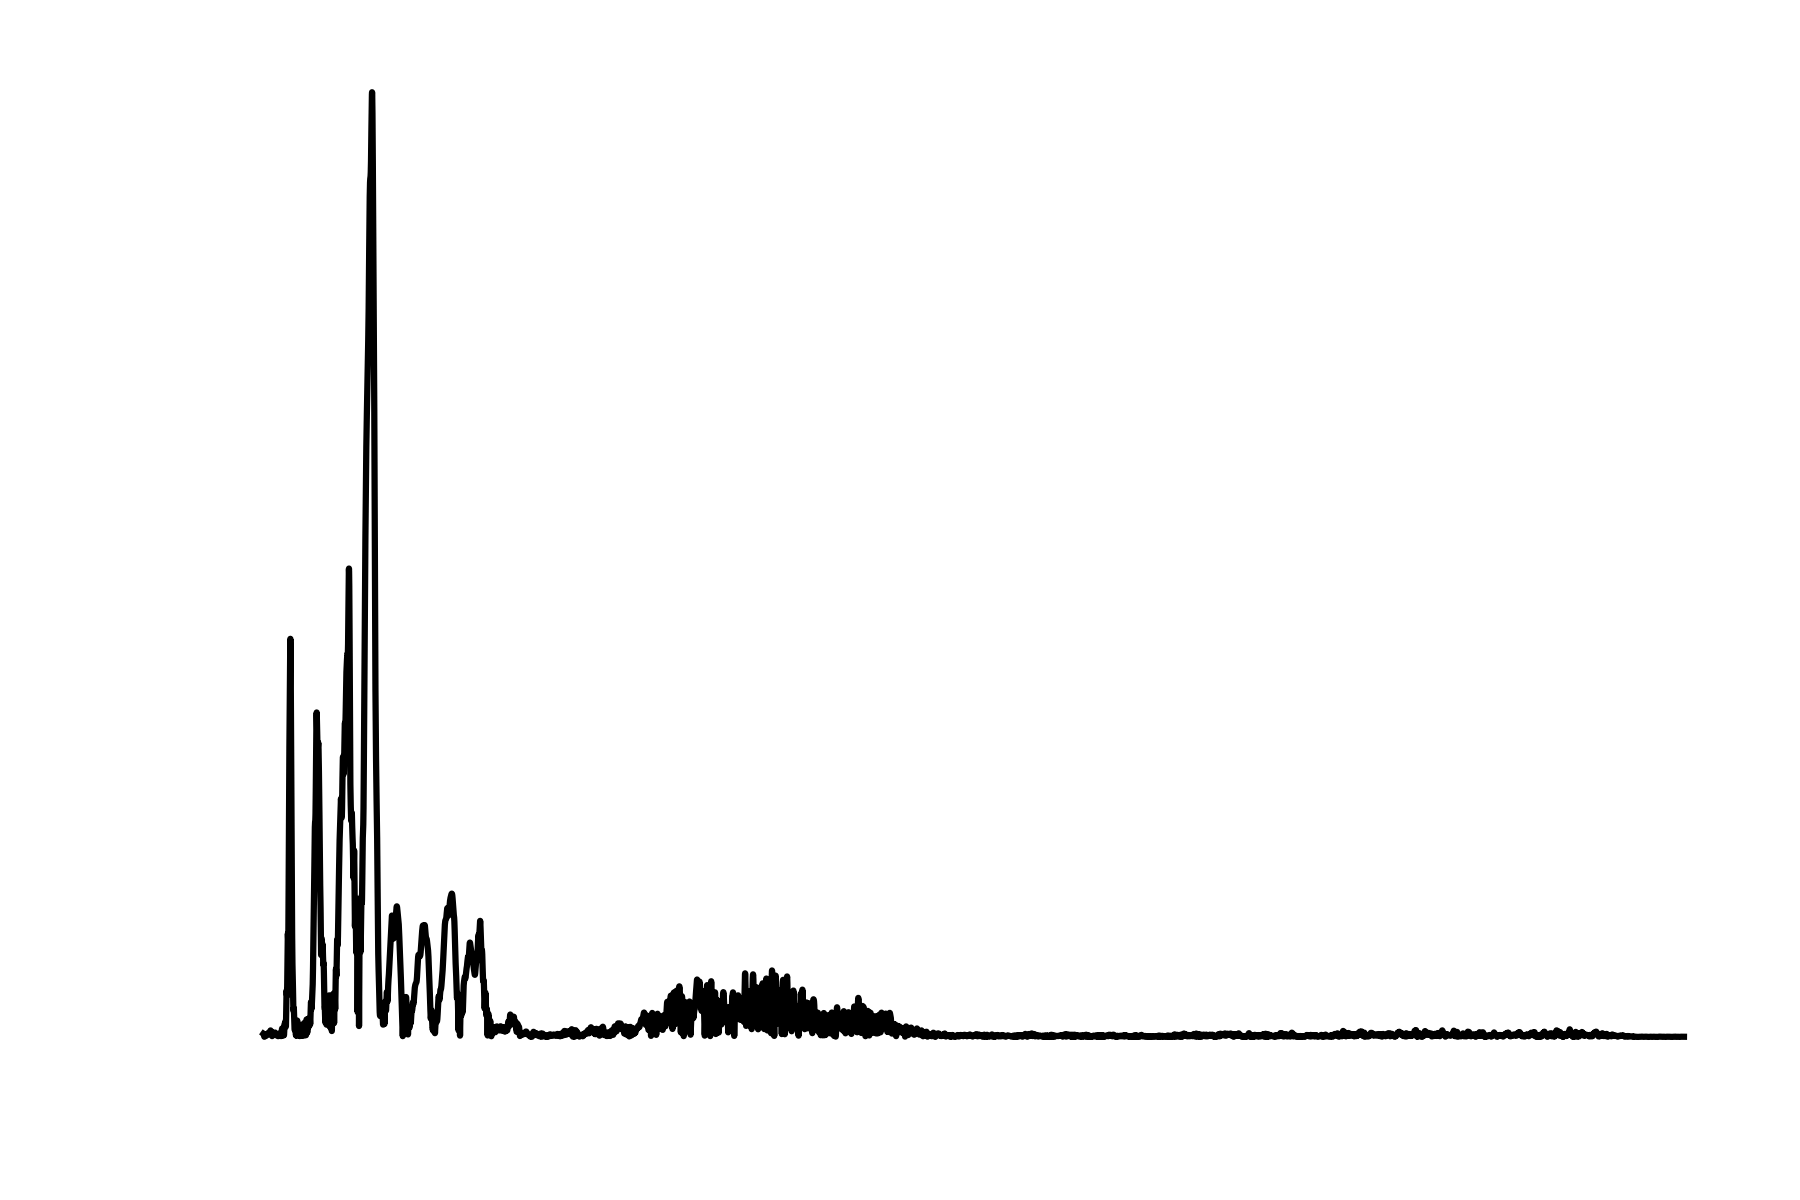
\includegraphics[width=52.5pt,height=35pt]{processing/py-freq_segment-0.png}};
%Image [id:dp3443235626087914]
\draw (575,183.33) node  {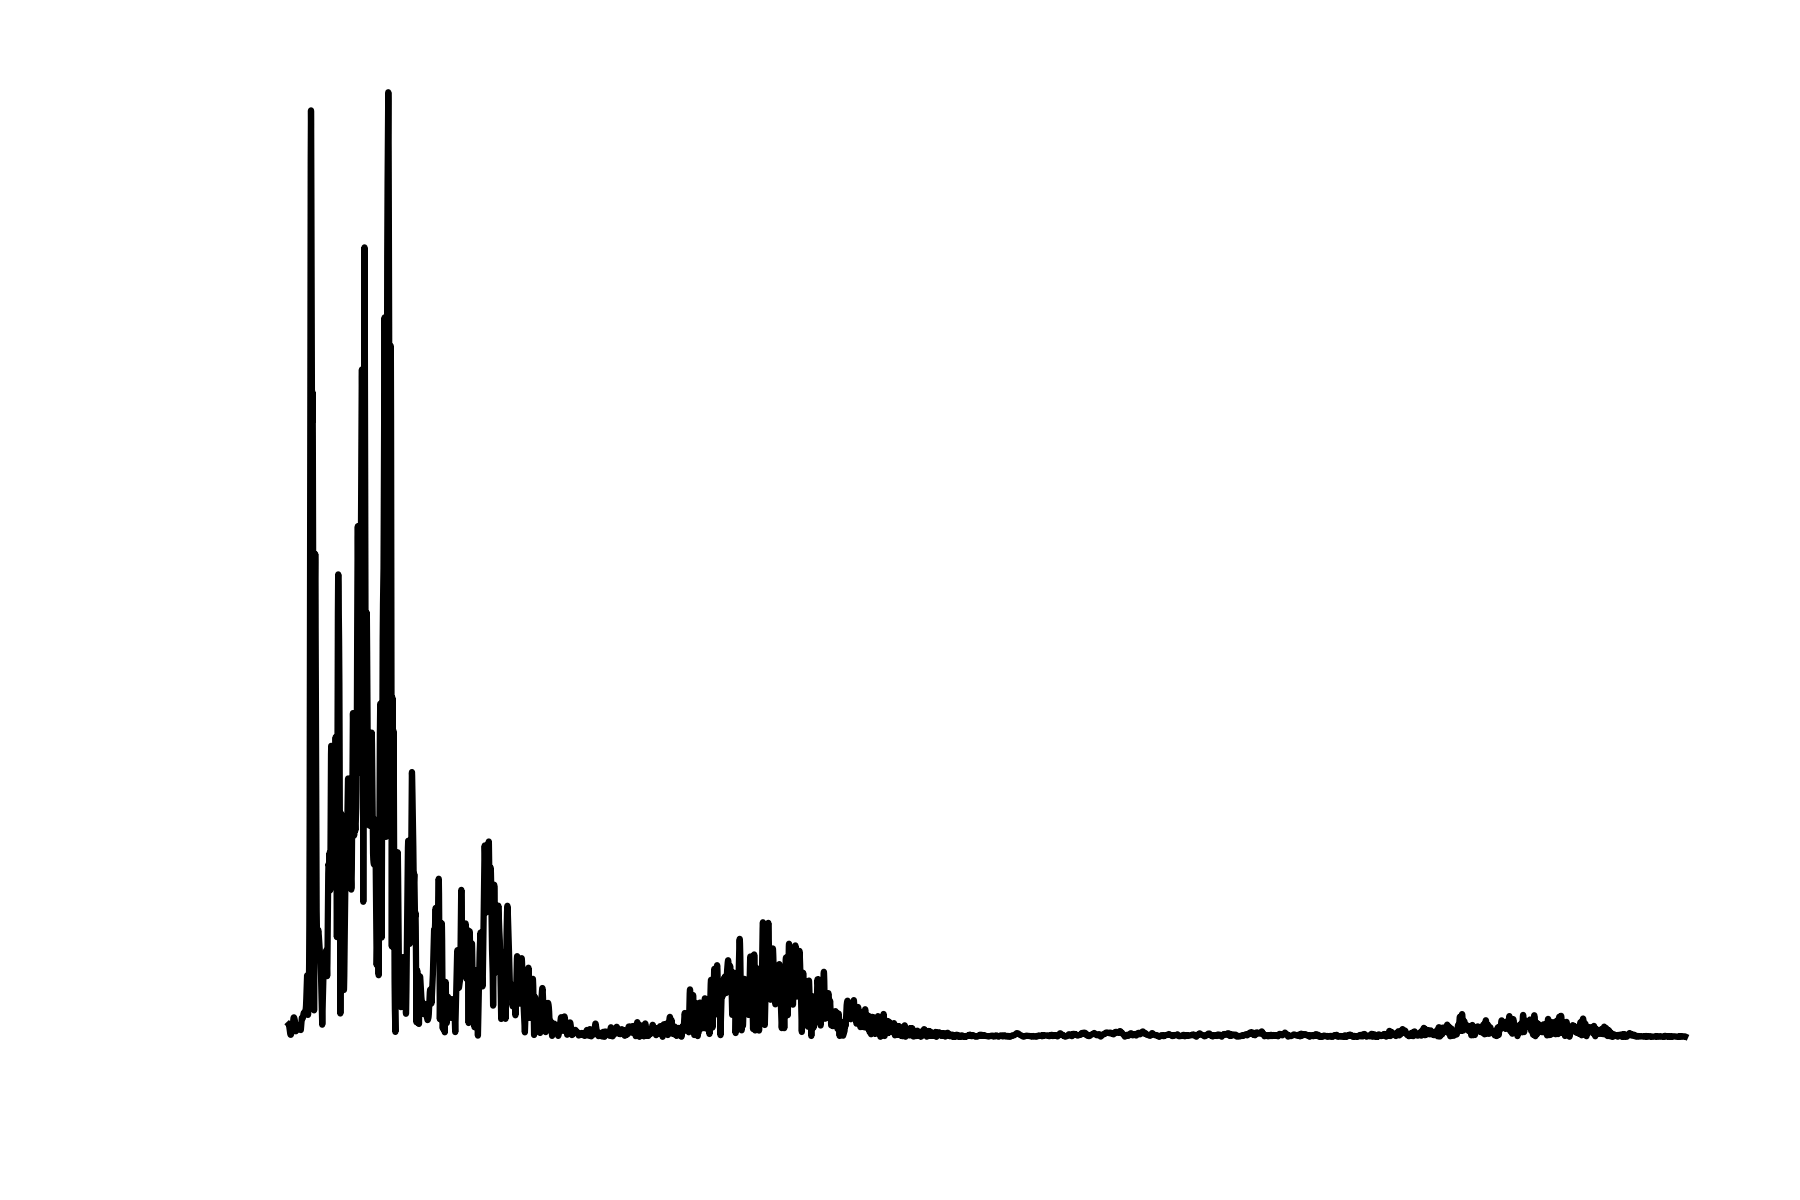
\includegraphics[width=52.5pt,height=35pt]{processing/py-freq_segment-1.png}};
%Image [id:dp2979363128108309]
\draw (105,146.5) node  {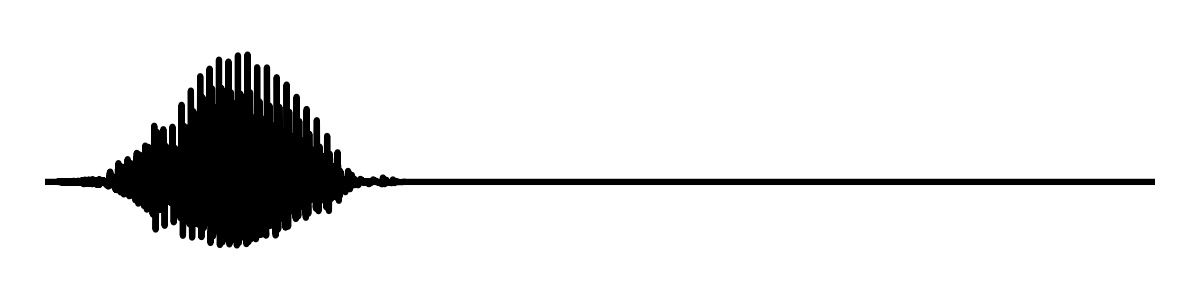
\includegraphics[width=105pt,height=26.25pt]{processing/py-time_segment-0.png}};
%Shape: Rectangle [id:dp4336148771055519]
\draw  [draw opacity=0][fill={rgb, 255:red, 255; green, 255; blue, 255 }  ,fill opacity=1 ] (60,180) -- (80,180) -- (80,200) -- (60,200) -- cycle ;
%Image [id:dp32871739431752567]
\draw (110,167) node  {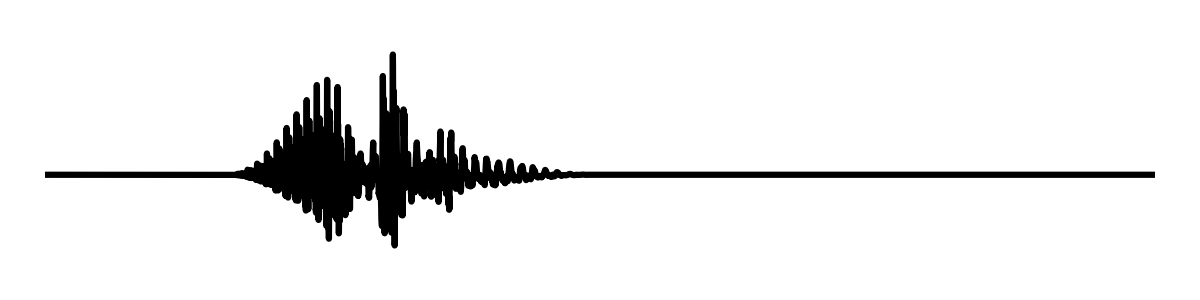
\includegraphics[width=105pt,height=30pt]{processing/py-time_segment-1.png}};
%Shape: Rectangle [id:dp8481412253766418]
\draw  [draw opacity=0][fill={rgb, 255:red, 255; green, 255; blue, 255 }  ,fill opacity=1 ] (40,160) -- (60,160) -- (60,200) -- (40,200) -- cycle ;
%Shape: Rectangle [id:dp03992819043895124]
\draw  [draw opacity=0][fill={rgb, 255:red, 255; green, 255; blue, 255 }  ,fill opacity=1 ] (120,140) -- (180,140) -- (180,180) -- (120,180) -- cycle ;
%Image [id:dp2476506667174908]
\draw (150.75,50.81) node  {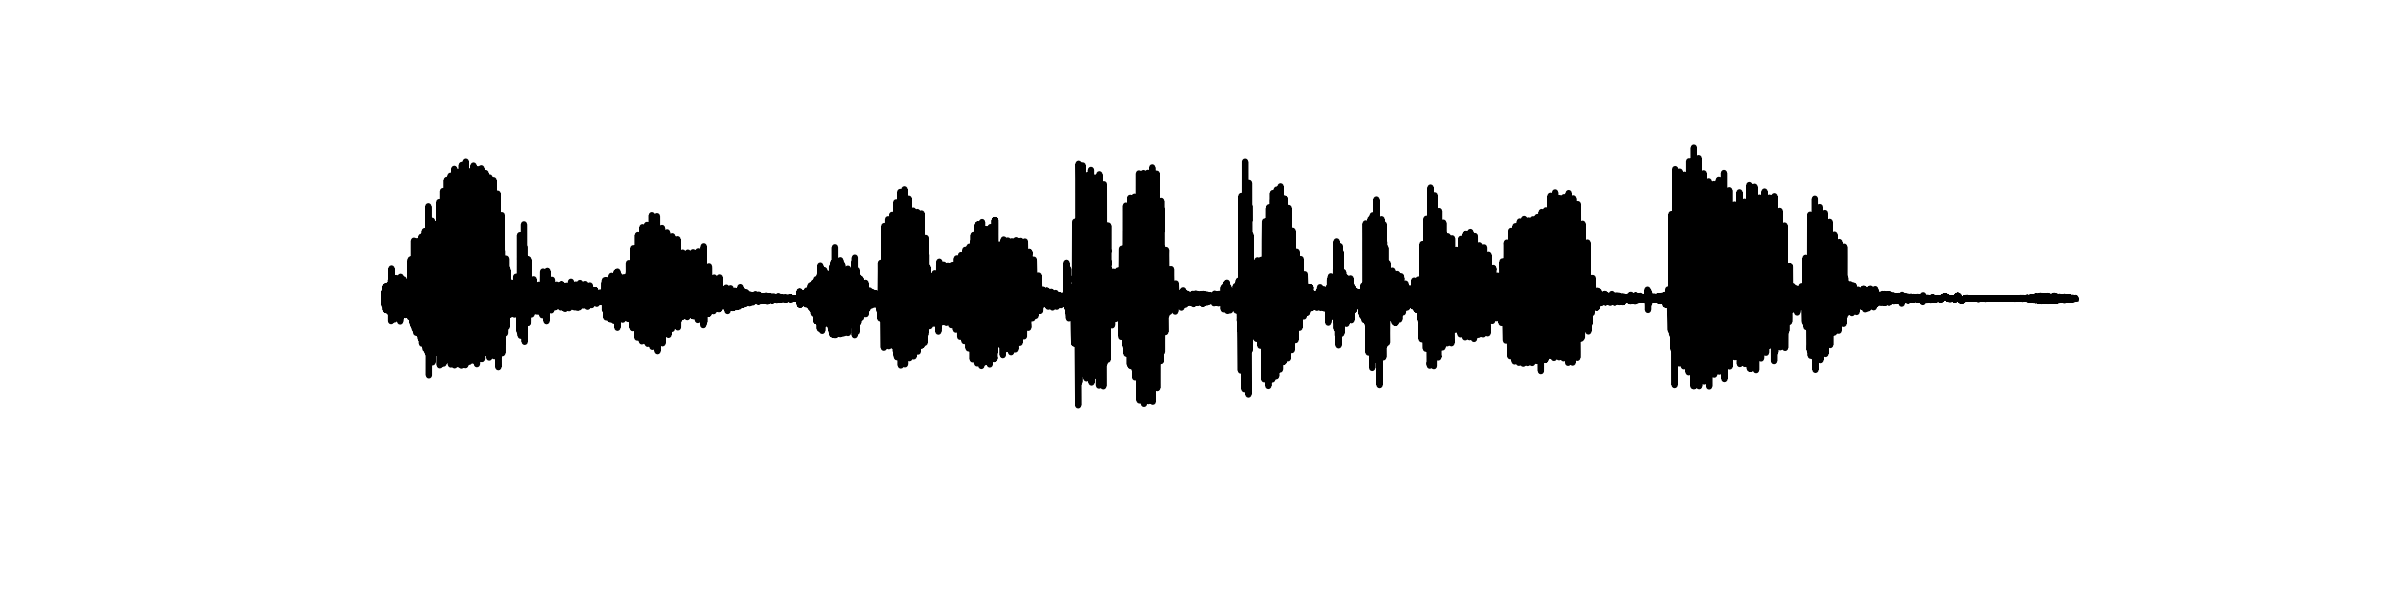
\includegraphics[width=244.88pt,height=61.22pt]{processing/py-waveform.png}};
%Shape: Rectangle [id:dp29156630749780055]
\draw  [draw opacity=0][fill={rgb, 255:red, 255; green, 255; blue, 255 }  ,fill opacity=1 ] (210,20) -- (330,20) -- (330,70) -- (210,70) -- cycle ;
%Image [id:dp4043877940980434]
\draw (525,130) node  {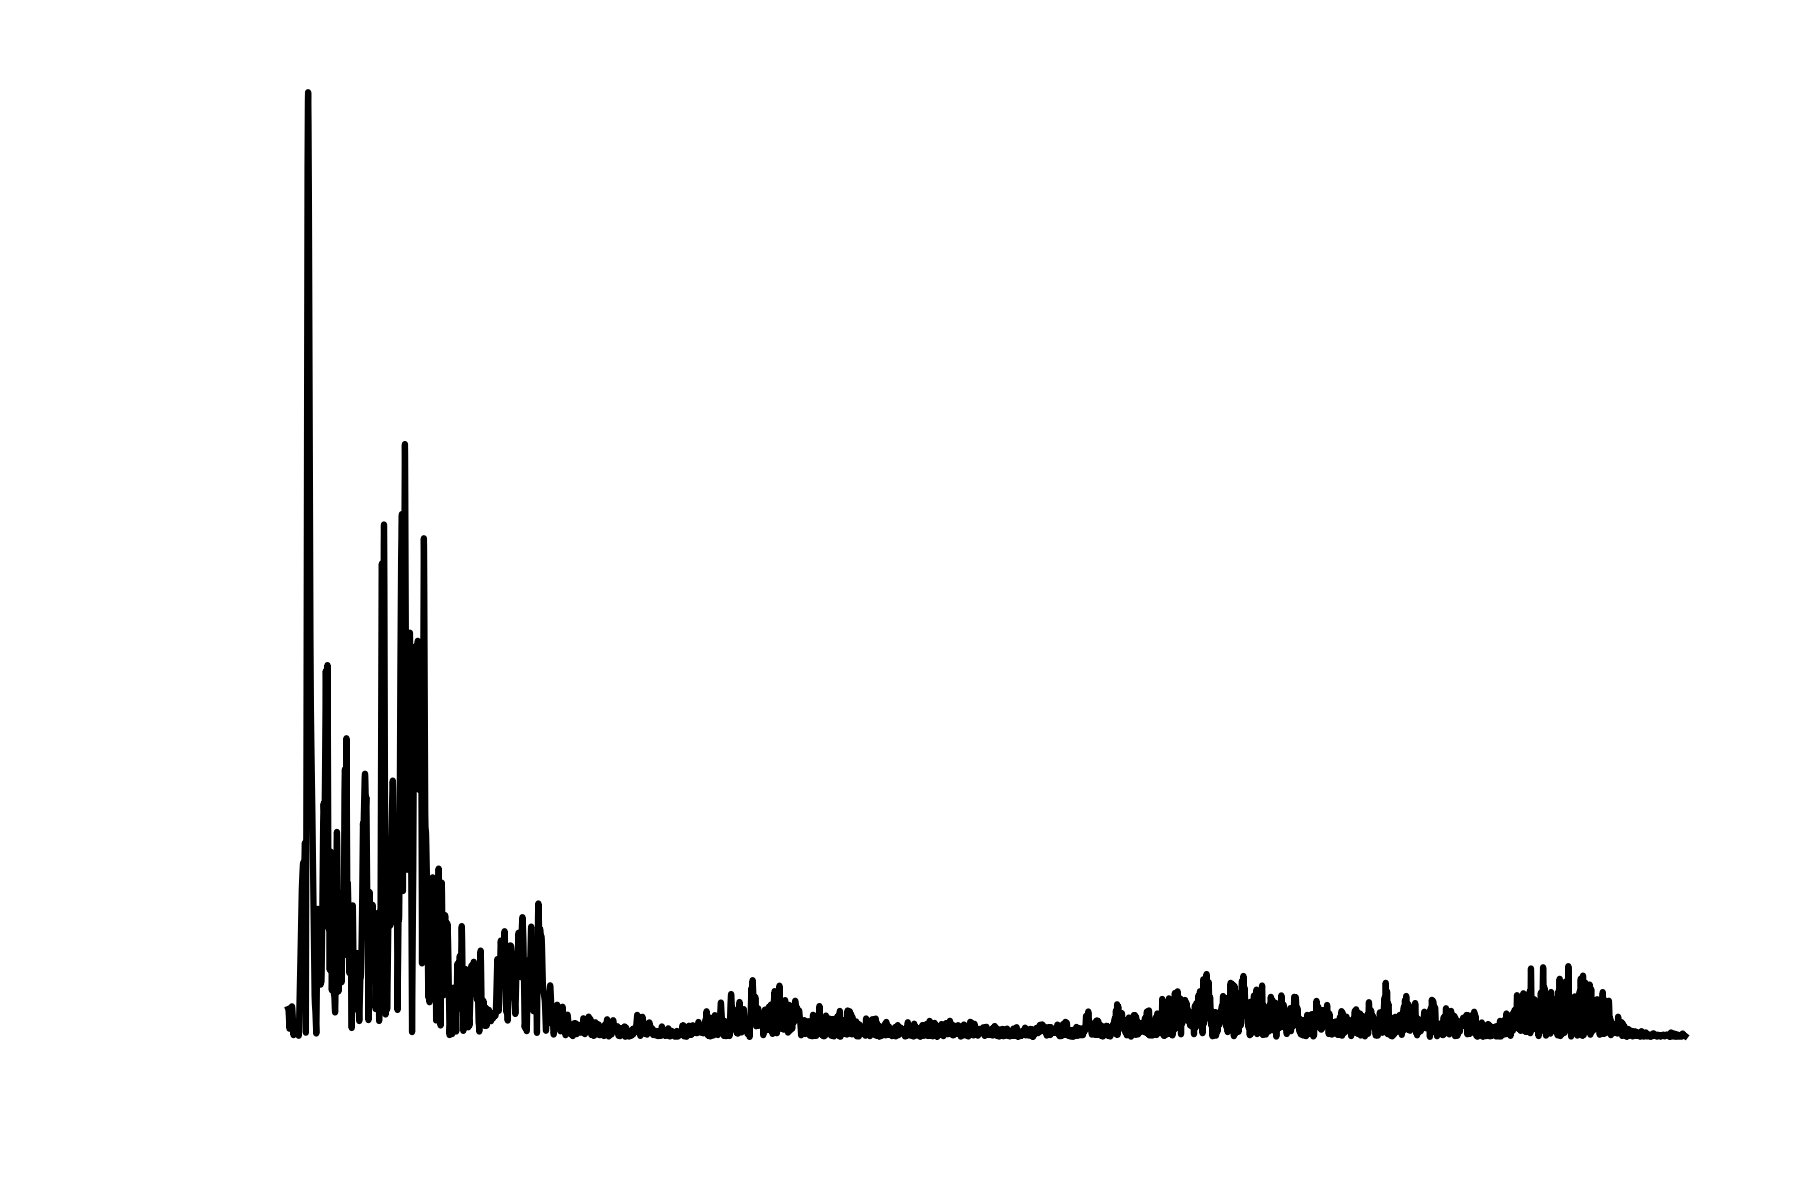
\includegraphics[width=67.5pt,height=45pt]{processing/py-freq_segment-2.png}};
%Shape: Rectangle [id:dp26622297727772126]
\draw  [draw opacity=0][fill={rgb, 255:red, 255; green, 255; blue, 255 }  ,fill opacity=1 ] (100,140) -- (120,140) -- (120,160) -- (100,160) -- cycle ;
%Image [id:dp8105828866624712]
\draw (105,198.5) node  {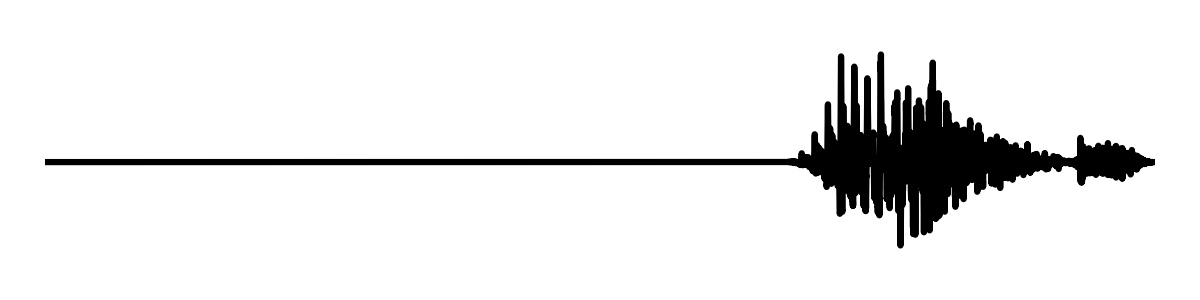
\includegraphics[width=105pt,height=26.25pt]{processing/py-time_segment-2.png}};
%Shape: Rectangle [id:dp6067652569911224]
\draw  [draw opacity=0][fill={rgb, 255:red, 255; green, 255; blue, 255 }  ,fill opacity=1 ] (40,190) -- (120,190) -- (120,210) -- (40,210) -- cycle ;
%Straight Lines [id:da9676641234627033]
\draw [color={rgb, 255:red, 128; green, 128; blue, 128 }  ,draw opacity=1 ]   (110,150) -- (478,150) ;
\draw [shift={(480,150)}, rotate = 180] [color={rgb, 255:red, 128; green, 128; blue, 128 }  ,draw opacity=1 ][line width=0.75]    (4.37,-1.32) .. controls (2.78,-0.56) and (1.32,-0.12) .. (0,0) .. controls (1.32,0.12) and (2.78,0.56) .. (4.37,1.32)   ;
%Straight Lines [id:da16098226613158673]
\draw [color={rgb, 255:red, 128; green, 128; blue, 128 }  ,draw opacity=1 ]   (130,170) -- (498,170) ;
\draw [shift={(500,170)}, rotate = 180] [color={rgb, 255:red, 128; green, 128; blue, 128 }  ,draw opacity=1 ][line width=0.75]    (4.37,-1.32) .. controls (2.78,-0.56) and (1.32,-0.12) .. (0,0) .. controls (1.32,0.12) and (2.78,0.56) .. (4.37,1.32)   ;
%Straight Lines [id:da11005264782971791]
\draw [color={rgb, 255:red, 128; green, 128; blue, 128 }  ,draw opacity=1 ]   (190,200) -- (528,200) ;
\draw [shift={(530,200)}, rotate = 180] [color={rgb, 255:red, 128; green, 128; blue, 128 }  ,draw opacity=1 ][line width=0.75]    (4.37,-1.32) .. controls (2.78,-0.56) and (1.32,-0.12) .. (0,0) .. controls (1.32,0.12) and (2.78,0.56) .. (4.37,1.32)   ;
%Shape: Square [id:dp8422681084136312]
\draw  [color={rgb, 255:red, 255; green, 255; blue, 255 }  ,draw opacity=1 ][fill={rgb, 255:red, 80; green, 227; blue, 194 }  ,fill opacity=1 ] (510,65) -- (520,65) -- (520,75) -- (510,75) -- cycle ;
%Shape: Square [id:dp6895251706790707]
\draw  [color={rgb, 255:red, 255; green, 255; blue, 255 }  ,draw opacity=1 ][fill={rgb, 255:red, 248; green, 231; blue, 28 }  ,fill opacity=1 ] (510,30) -- (520,30) -- (520,40) -- (510,40) -- cycle ;
%Shape: Square [id:dp8371453826772035]
\draw  [color={rgb, 255:red, 255; green, 255; blue, 255 }  ,draw opacity=1 ][fill={rgb, 255:red, 245; green, 166; blue, 35 }  ,fill opacity=1 ] (510,20) -- (520,20) -- (520,30) -- (510,30) -- cycle ;
%Shape: Square [id:dp4704612801462672]
\draw  [color={rgb, 255:red, 255; green, 255; blue, 255 }  ,draw opacity=1 ][fill={rgb, 255:red, 208; green, 2; blue, 27 }  ,fill opacity=1 ] (510,10) -- (520,10) -- (520,20) -- (510,20) -- cycle ;
%Shape: Square [id:dp04259158217783243]
\draw  [color={rgb, 255:red, 255; green, 255; blue, 255 }  ,draw opacity=1 ][fill={rgb, 255:red, 248; green, 231; blue, 28 }  ,fill opacity=1 ] (530,10) -- (540,10) -- (540,20) -- (530,20) -- cycle ;
%Shape: Square [id:dp8235422331679458]
\draw  [color={rgb, 255:red, 255; green, 255; blue, 255 }  ,draw opacity=1 ][fill={rgb, 255:red, 80; green, 227; blue, 194 }  ,fill opacity=1 ] (530,20) -- (540,20) -- (540,30) -- (530,30) -- cycle ;
%Shape: Square [id:dp7304739651989954]
\draw  [color={rgb, 255:red, 255; green, 255; blue, 255 }  ,draw opacity=1 ][fill={rgb, 255:red, 128; green, 128; blue, 128 }  ,fill opacity=1 ] (530,30) -- (540,30) -- (540,40) -- (530,40) -- cycle ;
%Shape: Square [id:dp4388945574586607]
\draw  [color={rgb, 255:red, 255; green, 255; blue, 255 }  ,draw opacity=1 ][fill={rgb, 255:red, 126; green, 211; blue, 33 }  ,fill opacity=1 ] (530,65) -- (540,65) -- (540,75) -- (530,75) -- cycle ;
%Shape: Square [id:dp9653722203138573]
\draw  [color={rgb, 255:red, 255; green, 255; blue, 255 }  ,draw opacity=1 ][fill={rgb, 255:red, 248; green, 231; blue, 28 }  ,fill opacity=1 ] (570,30) -- (580,30) -- (580,40) -- (570,40) -- cycle ;
%Shape: Square [id:dp981513589679916]
\draw  [color={rgb, 255:red, 255; green, 255; blue, 255 }  ,draw opacity=1 ][fill={rgb, 255:red, 208; green, 2; blue, 27 }  ,fill opacity=1 ] (570,20) -- (580,20) -- (580,30) -- (570,30) -- cycle ;
%Shape: Square [id:dp8950073186581587]
\draw  [color={rgb, 255:red, 255; green, 255; blue, 255 }  ,draw opacity=1 ][fill={rgb, 255:red, 80; green, 227; blue, 194 }  ,fill opacity=1 ] (570,10) -- (580,10) -- (580,20) -- (570,20) -- cycle ;
%Shape: Square [id:dp1665737624049748]
\draw  [color={rgb, 255:red, 255; green, 255; blue, 255 }  ,draw opacity=1 ][fill={rgb, 255:red, 126; green, 211; blue, 33 }  ,fill opacity=1 ] (570,65) -- (580,65) -- (580,75) -- (570,75) -- cycle ;
%Straight Lines [id:da7233973673270127]
\draw [color={rgb, 255:red, 128; green, 128; blue, 128 }  ,draw opacity=1 ]   (60,110) -- (60,128) ;
\draw [shift={(60,130)}, rotate = 270] [color={rgb, 255:red, 128; green, 128; blue, 128 }  ,draw opacity=1 ][line width=0.75]    (4.37,-1.32) .. controls (2.78,-0.56) and (1.32,-0.12) .. (0,0) .. controls (1.32,0.12) and (2.78,0.56) .. (4.37,1.32)   ;
%Straight Lines [id:da6893975030077206]
\draw [color={rgb, 255:red, 128; green, 128; blue, 128 }  ,draw opacity=1 ]   (220,50) -- (478,50) ;
\draw [shift={(480,50)}, rotate = 180] [color={rgb, 255:red, 128; green, 128; blue, 128 }  ,draw opacity=1 ][line width=0.75]    (4.37,-1.32) .. controls (2.78,-0.56) and (1.32,-0.12) .. (0,0) .. controls (1.32,0.12) and (2.78,0.56) .. (4.37,1.32)   ;
%Straight Lines [id:da7882799041842373]
\draw [color={rgb, 255:red, 128; green, 128; blue, 128 }  ,draw opacity=1 ]   (514,140) -- (514,92) ;
\draw [shift={(514,90)}, rotate = 450] [color={rgb, 255:red, 128; green, 128; blue, 128 }  ,draw opacity=1 ][line width=0.75]    (4.37,-1.32) .. controls (2.78,-0.56) and (1.32,-0.12) .. (0,0) .. controls (1.32,0.12) and (2.78,0.56) .. (4.37,1.32)   ;
%Straight Lines [id:da0855776778601487]
\draw [color={rgb, 255:red, 128; green, 128; blue, 128 }  ,draw opacity=1 ]   (534,160) -- (534,92) ;
\draw [shift={(534,90)}, rotate = 450] [color={rgb, 255:red, 128; green, 128; blue, 128 }  ,draw opacity=1 ][line width=0.75]    (4.37,-1.32) .. controls (2.78,-0.56) and (1.32,-0.12) .. (0,0) .. controls (1.32,0.12) and (2.78,0.56) .. (4.37,1.32)   ;
%Straight Lines [id:da12659425796956003]
\draw [color={rgb, 255:red, 128; green, 128; blue, 128 }  ,draw opacity=1 ]   (574,190) -- (574,92) ;
\draw [shift={(574,90)}, rotate = 450] [color={rgb, 255:red, 128; green, 128; blue, 128 }  ,draw opacity=1 ][line width=0.75]    (4.37,-1.32) .. controls (2.78,-0.56) and (1.32,-0.12) .. (0,0) .. controls (1.32,0.12) and (2.78,0.56) .. (4.37,1.32)   ;
%Image [id:dp7783322035520386]
\draw (60,91.5) node  {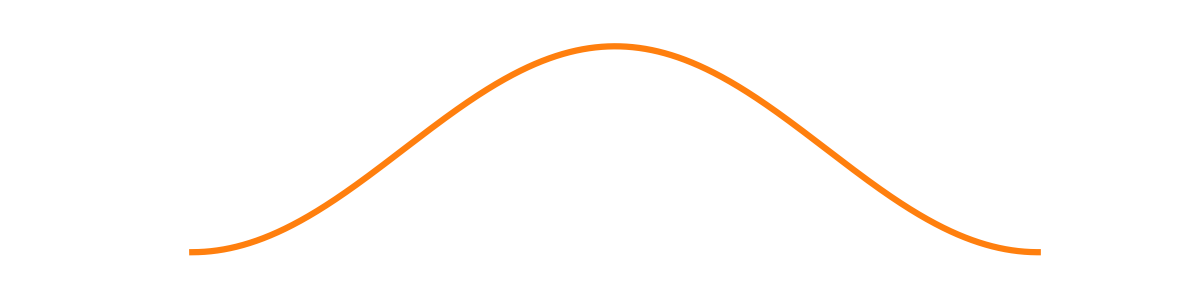
\includegraphics[width=45pt,height=18.75pt]{processing/py-window_hann.png}};
%Image [id:dp19952118090411974]
\draw (90,91.5) node  {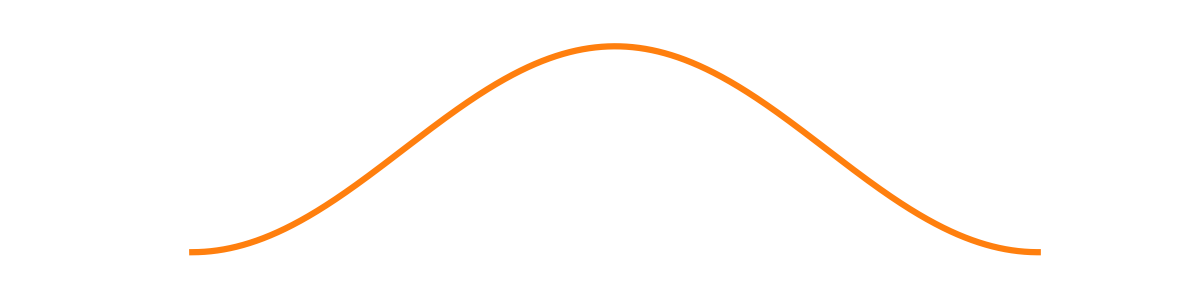
\includegraphics[width=45pt,height=18.75pt]{processing/py-window_hann.png}};
%Image [id:dp33944658963121455]
\draw (150,91.5) node  {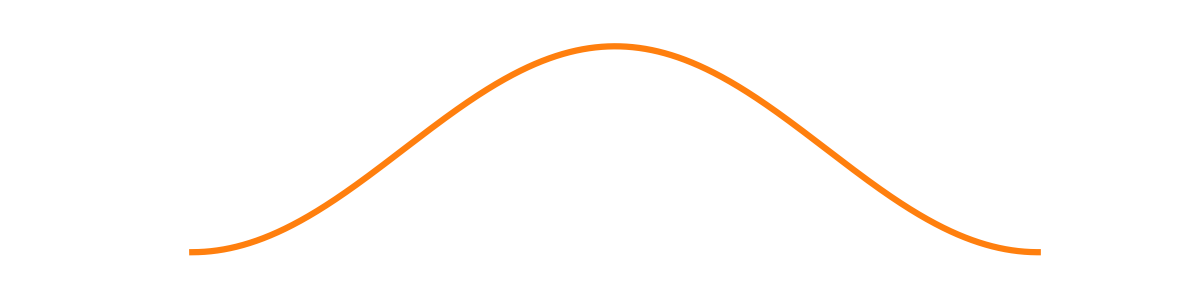
\includegraphics[width=45pt,height=18.75pt]{processing/py-window_hann.png}};
%Flowchart: Process [id:dp8413645612532185]
\draw  [draw opacity=0][fill={rgb, 255:red, 255; green, 255; blue, 255 }  ,fill opacity=1 ] (152.51,167.51) -- (152.49,172.51) -- (146.49,172.49) -- (146.51,167.49) -- cycle ;
%Flowchart: Process [id:dp7058794182815539]
\draw  [draw opacity=0][fill={rgb, 255:red, 255; green, 255; blue, 255 }  ,fill opacity=1 ] (86.5,152.5) -- (86.5,147.5) -- (92.5,147.5) -- (92.5,152.5) -- cycle ;
%Straight Lines [id:da3609616268595228]
\draw [color={rgb, 255:red, 128; green, 128; blue, 128 }  ,draw opacity=1 ]   (90,110) -- (90,158) ;
\draw [shift={(90,160)}, rotate = 270] [color={rgb, 255:red, 128; green, 128; blue, 128 }  ,draw opacity=1 ][line width=0.75]    (4.37,-1.32) .. controls (2.78,-0.56) and (1.32,-0.12) .. (0,0) .. controls (1.32,0.12) and (2.78,0.56) .. (4.37,1.32)   ;
%Flowchart: Process [id:dp9166675646225523]
\draw  [draw opacity=0][fill={rgb, 255:red, 255; green, 255; blue, 255 }  ,fill opacity=1 ] (152.51,147.51) -- (152.49,152.51) -- (146.49,152.49) -- (146.51,147.49) -- cycle ;
%Straight Lines [id:da3140233984836672]
\draw [color={rgb, 255:red, 128; green, 128; blue, 128 }  ,draw opacity=1 ]   (150,110) -- (150,178) ;
\draw [shift={(150,180)}, rotate = 270] [color={rgb, 255:red, 128; green, 128; blue, 128 }  ,draw opacity=1 ][line width=0.75]    (4.37,-1.32) .. controls (2.78,-0.56) and (1.32,-0.12) .. (0,0) .. controls (1.32,0.12) and (2.78,0.56) .. (4.37,1.32)   ;

% Text Node
\draw (323.74,169.4) node [anchor=north west][inner sep=0.75pt]  [font=\tiny,rotate=-45.3]  {$\dotsc $};
% Text Node
\draw (110,79.4) node [anchor=north west][inner sep=0.75pt]  [font=\footnotesize,color={rgb, 255:red, 245; green, 166; blue, 35 }  ,opacity=1 ]  {$\dotsc $};
% Text Node
\draw (301,37) node [anchor=north west][inner sep=0.75pt]  [font=\scriptsize] [align=left] {STFT};
% Text Node
\draw (290,137) node [anchor=north west][inner sep=0.75pt]  [font=\scriptsize] [align=left] {DFT};
% Text Node
\draw (307,157) node [anchor=north west][inner sep=0.75pt]  [font=\scriptsize] [align=left] {DFT};
% Text Node
\draw (327,187) node [anchor=north west][inner sep=0.75pt]  [font=\scriptsize] [align=left] {DFT};
% Text Node
\draw (516,126) node [anchor=north west][inner sep=0.75pt]  [font=\tiny,rotate=-270] [align=left] {Vector};
% Text Node
\draw (536,126) node [anchor=north west][inner sep=0.75pt]  [font=\tiny,rotate=-270] [align=left] {Vector};
% Text Node
\draw (576,126) node [anchor=north west][inner sep=0.75pt]  [font=\tiny,rotate=-270] [align=left] {Vector};
% Text Node
\draw (55,72.4) node [anchor=north west][inner sep=0.75pt]  [font=\tiny,color={rgb, 255:red, 245; green, 166; blue, 35 }  ,opacity=1 ]  {$\times $};
% Text Node
\draw (543,26.4) node [anchor=north west][inner sep=0.75pt]    {$\dotsc $};
% Text Node
\draw (561.4,65) node [anchor=north west][inner sep=0.75pt]  [rotate=-270]  {$\dotsc $};
% Text Node
\draw (521.4,65) node [anchor=north west][inner sep=0.75pt]  [rotate=-270]  {$\dotsc $};
% Text Node
\draw (501.4,65) node [anchor=north west][inner sep=0.75pt]  [rotate=-270]  {$\dotsc $};
% Text Node
\draw (86,72.4) node [anchor=north west][inner sep=0.75pt]  [font=\tiny,color={rgb, 255:red, 245; green, 166; blue, 35 }  ,opacity=1 ]  {$\times $};
% Text Node
\draw (145,72.4) node [anchor=north west][inner sep=0.75pt]  [font=\tiny,color={rgb, 255:red, 245; green, 166; blue, 35 }  ,opacity=1 ]  {$\times $};


\end{tikzpicture}

    \end{fullwidth}
\end{figure}


\subsection{The final model}\label{subsec:processing:model:stft}
The model \eqref{eq:processing:discreteModel} shows how in practice the RIRs are treated in the frequency-domain.
However this does not generalize straightforwardly to the time-frequency domain:
it depends on the length of the filter \wrt/ to the length of the analysis window on of the \STFT/.
Issues arise with ``long'' filters, which are common in highly reverberant or time-varying scenarios.
To circumvent this issue, the \textit{convolutional STFT} for arbitrary window functions have been proposed\sidenote{%
It translates the time-domain convolution into inter-frame and inter-band convolutions, rather than pointwise multiplication of Fourier transforms.
}~\citeonly{gilloire1992adaptive}.
Although mathematically exact, it is computationally and memory intensive.

In this thesis, we will assume that the filter length is shorter than the analysis window length.
In the literature, this is known as the \textit{narrowband approximation}, namely the time-domain filtering can be approximated by complex-valued multiplication in each time-frequency bin $[l,k]$:
\begin{equation}\label{eq:processing:narrow}
    \IMGS_j[l,k] \approx \hat{\FLTS}[k] \SRC_j[l,k]
    ,
\end{equation}
where the $\hat{\FLTS}_j[k] = \ktranspose{\klist{\hat{\flt}_{1j}[k], \cdots, \hat{\flt}_{Ij}[k]}}$ is the $I \times 1$ vector of the \RTF/s for source $j$.
It is sometimes practical to concatenate all these vectors into an $I \times J$ matrix $\hat{\FLTSS}[k] = \klist{\FLTS_1(f),\cdots,\FLTS_J(f)}$ called \textit{mixing matrix}.

With the above notation and considerations, mixing process including noise terms can be written in the \STFT/ domain compactly as:
\begin{equation}\label{eq:processing:model:stfs}
    \MICS[l,k] = \FLTSS[l,k] \SRCS[l,k] + \bsU[l,k]
\end{equation}
where $\bsU[l,k] = \bsN[l,k] + \boldsymbol{\varepsilon}(l,k)$ includes the contribution of both diffuse noise sources, modeling and measurement errors.

% The above equation can be seen as a \textit{deterministic} parametrization of the mixing process and it does not consider a statistical description
% of the reverberation. In fact it the filter

% \newthoughtpar{The spatial quadratic STFT transform}
% \begin{equation}
%     \cov_{\mics}[l,k] = \bbE \klist{\mics[l,k]\khermitian{\mics[l,k]}}
% \end{equation}

\section{Other (room) impulse response spectral models}\label{sec:processing:rirmodels}
\RIRs/ are complicated quantities to model, compute and estimate.
The representations of the \RIR/ discussed so far explicitly models early echoes and reverberation deterministically.
Furthermore, alternative models are common in the audio processing literature.

\subsection{Steering vector model}\label{subsec:processing:steering}
In the absence of echoes and reverberation, namely assuming free-field propagation,
the \RIRs/ simplify to \textit{steering vectors}, namely the DFT of~\cref{eq:acoustics:greenFreeTime}:
\begin{equation}\label{eq:processing:steering}
    \bsD_{j}[k] = \klist{\frac{1}{4 \pi \distMicSrc_{1j}} \cste^{-\csti 2 \pi f_k \distMicSrc_{1j} / c},
                            \cdots,
                            \frac{1}{4 \pi \distMicSrc_{Ij}} \cste^{-\csti 2 \pi f_k \distMicSrc_{Ij} / c},
                    }
\end{equation}
Furthermore, assuming far-field regimes, the microphone-to-source distance $\distMicSrc_{ij}$ is larger than the
inter-microphone distance $d_{ii'}$ making the attenuation factors $\sfrac{1}{4 \pi \distMicSrc_{ij}}$ approximately equal, hence ignored.

\subsection{Relative transfer function and interchannel models}\label{subsec:processing:rtf}
Let us consider now only two channels and only one source signal in the model~\cref{eq:processing:model:stfs}.
Dropping the dependency on $j$ for readability and taking the first channel as reference, the \ReTFdef/ associated to the $i$-th channel is defined as
the element-wise ratio of the (D)FTs of the two filters~\citeonly{gannot2001signal}
\begin{equation}\label{eq:processing:rtf}
    \hat{G}_i[k] = \frac{\hat{\FLT}_i[k]}{\hat{\FLT}_1[k]}
    .
\end{equation}

The continuous-time domain counterpart is called as \ReIRdef/ and can be interpreted as the filter ``transforming'' the $i$-th impulse response into the one of the reference channel.
Considering the noisy observation $\tilde{x}_i$ and $\tilde{x}_1$, their signals can be re-written in term of $\tilde{g}_i$ as follows
\begin{equation}
    \begin{matrix}
    \begin{cases}
        \tilde{\mic}_1 = \tilde{\rir}_1 \convCont \tilde{s} + \tilde{\allNoise}_1 \\
        \tilde{\mic}_i = \tilde{\rir}_i \convCont \tilde{s} + \tilde{\allNoise}_i
    \end{cases} & \kto  & \begin{cases}
        \tilde{\mic}_1 = \tilde{\rir}_1 \convCont \tilde{s} + \tilde{\allNoise}_1 \\
        \tilde{\mic}_i = \tilde{\rtf}_i \convCont \tilde{\rir}_i \convCont \tilde{s} + \tilde{\allNoise}_i
    \end{cases}
    \end{matrix}
    .
\end{equation}
Notice that $\tilde{\rir}_i = \tilde{\rtf}_i \convCont \tilde{\rir}_1$ corresponds to~\cref{eq:processing:rtf} in the frequency domain.
Moreover although the real-world \RIRs/ $h_1$ and $h_i$ are causal, their \ReTF/ needs not be so.

The \ReTFs/ benefits of several interesting properties that will be of fundamental importance for this thesis.
In particular:
\begin{itemize}
    \item the \ReTF/ associated to the reference channel ($i = 1$) is equal to $1$ for each frequency bin $k$.
    \item The problem of estimating the \ReTF/ can be considered ``easier'' than \RIRs/ estimation.
    In fact, in the noiseless case, it holds that $\tilde{\mic}_i = \tilde{\rtf}_i \convCont \tilde{\mic}_1$.
    \item The \ReTFs/ encode properties of the related impulse responses and there are many efficient methods to estimate them\sidenote{%
        In~\cref{ch:brioche} methods for estimation the ReTF will be discussed
    }.
    Therefore, it may be used as a proxy for the estimations of (components of) \RIRs/.
    \item A \RIR/ can be seen as a special case of \ReTF/ where the non-reference microphone is a virtual one whose
    output is the original (non-spatial) source signal $\src$. In fact, if $\rir_1 = \delta$ then $\rtf_i = \rir_i$\sidenote{%
    In practice this virtual microphone is sometimes substituted by a microphone that is very close to the source.}.
    \item As discussed below, \ReTFs/ simplify to special steering vectors in free- and far-field conditions, which have interesting geometrical properties.
\end{itemize}

In the general case of multiple microphone arrays ($I>2$) and multiple sources, the vector of \ReTFs/
$\boldsymbol{G}_j[k] = \ktranspose{\klist{\hat{G}_ {1j}[k], \cdots, \hat{G}_{Ij}[k]}}$
for the $j$-th source is defined as
\begin{equation}
    \hat{\bsG}_j[k] = \frac{1}{\hat{G}_{1j}[k]} \hat{\bsG}_j[k]
    .
\end{equation}


\newthought{The relative steering vectors} are obtained by combining~\cref{eq:processing:steering,eq:processing:rtf} as
\begin{equation}\label{eq:processing:relativesteering}
    \hat{\bsD}_{j}[k] = \klist{
                         1,
                         \cste^{-\csti 2 \pi f_k (\distMicSrc_{2j}-\distMicSrc_{i'j}) / \speedOfSound},
                         \ldots,
                         \cste^{-\csti 2 \pi f_k (\distMicSrc_{Ij}-\distMicSrc_{i'j}) / \speedOfSound}
                    }
\end{equation}
where $(\distMicSrc_{ij}-\distMicSrc_{1j}) / \speedOfSound$ is the \TDOA/ between the $i$-th and the reference microphones.
The \TDOAs/ will be the protagonists of~\cref{chap:mirage} as they are fundamental quantities for sound source localization.

\newthought{\ReTFs/ estimate}
Since~\citeonly{gannot2001signal}, many methods have been proposed to estimated it.
A na\:ive way to estimated the \ReTF/ is perform the ratio between the \DFT/ of microphone pairs.
Despite its simplicity, this methods yield estimated


\newthought{In the context of spatial auditory perception} and \CASA/, the \ReTF/ is related to the \textit{interchannel cues}\sidenote{%
sometimes refers to as \textit{interaural cues} when a stress is put on the fact that the two ears are considered as receivers}.
In fact, the \ReTFs/ encodes the so-called \ILD/ and the \IPD/
\begin{equation}
    \begin{aligned}
        \ild_{ij}[k] &= 20 \log_{10} \magnitudeOf{\rtf[k]} & [\si{\dB}]\\
        \ipd_{ij}[k] &= \phaseOf{\rtf[k]} \mathspace       & [\si{\radian}]
    \end{aligned}
\end{equation}

As shown in~\cref{fig:processing:ildipd}, the \ILD/ and the \IPD/ cluster around the direct path, associated to the direct path component.
However early echoes and reverberation make them significantly diverge.

\begin{figure}[b]
    \begin{fullwidth}
        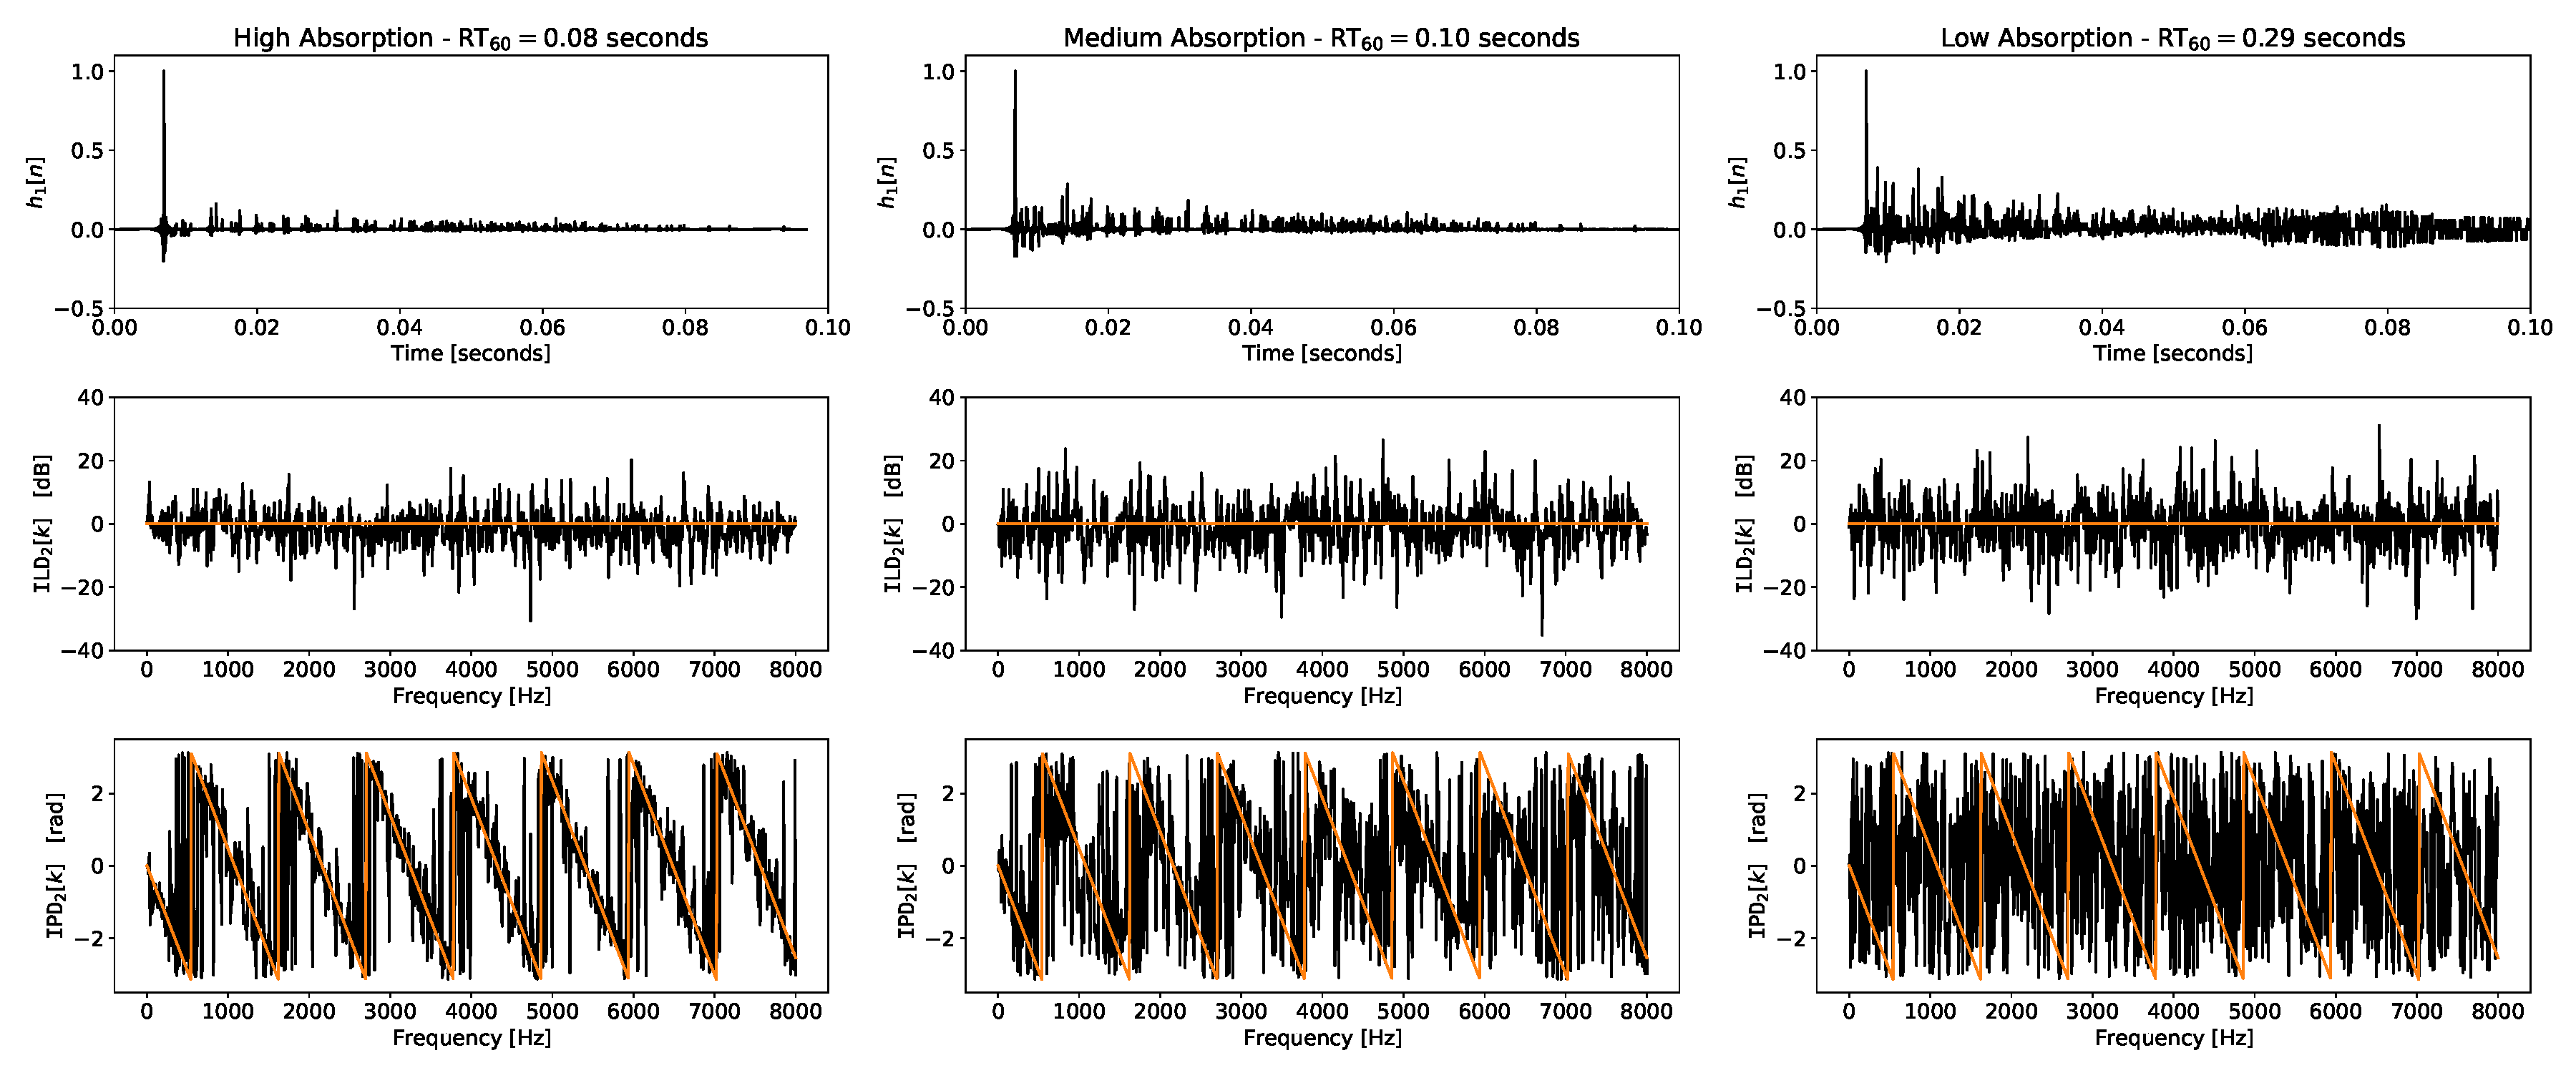
\includegraphics[width=\linewidth+\marginparsep]{processing/py-rtf.pdf}
        \caption{
            \RIR/, \ILD/ and \IPD/ corresponding to the pair of synthetic impulse responses of~\cref{fig:acoustics:rir} for different absorption conditions.
            Orange lines denote the theoretical far- and free- field \ILD/ and \IPD/ as defined by the relative steering vectors of~\cref{eq:processing:relativesteering}
        }\label{fig:processing:ildipd}
    \end{fullwidth}
\end{figure}


% \subsection{Probabilistic and Full-rank covariance model}
% For certain applications, it is more common to assume a statistical point of view, known as the \textit{Local Gaussian Model}\cite{}.
% Assume that the source STFT coefficients sj(n, f) have a zero-mean nonstationary Gaussian distribution with variance σ2
% sj (n, f), and they are all independent source-,
% frame- and frequency-wise (i.e., over j, n and f)